%% ------------------------------------------------------------
%% TITLE:     Digital Biosignal Processing - Notes
%% AUTHOR:    BINGHUAN W LI (Dept. Chemical Eng/Bio Eng, Imperial)
%% COMPILED:  XeLaTeX with TeX Live version 2023
%% LICENSE:   This work is licensed under a Creative Commons Attribution-NonCommercial 4.0 International License.
%% ------------------------------------------------------------

% Version History:
% v1.0  - 2024-11 - Initial draft

\documentclass[12pt,a4paper]{article}
\usepackage[margin=2.5cm]{geometry}

\usepackage[slantedGreek]{mathptmx}
\usepackage{fontspec}
    \setmainfont{Times New Roman}

\usepackage{tabularx}
\usepackage{booktabs}
\usepackage{wrapfig}
\usepackage{graphicx, float, subcaption}
\usepackage[export]{adjustbox}
\usepackage{enumitem}
\renewcommand\tabularxcolumn[1]{m{#1}}

\usepackage{amsmath,amsfonts,amssymb}
\usepackage{mathrsfs,mathtools} 

\usepackage[font={small,it}]{caption}
    \captionsetup[figure]{labelfont={sc},name={Fig.}}

\usepackage[most]{tcolorbox}
    \tcbuselibrary{breakable}
    
\usepackage{tikzducks}
\usepackage[european]{circuitikz}
\usepackage{tikz}
    \usetikzlibrary{arrows}

\usepackage{sidecap}
\usepackage{cancel}
\usepackage{multicol}
\usepackage{fontawesome}

\usepackage[]{mdframed}

\usepackage{fancyhdr}
    \pagestyle{fancy}
    \fancyhf{}
    \lhead{\textit{\leftmark}}
    \lfoot{\textbf{\thepage}}

% define colors
\usepackage{xcolor}
    \definecolor{navy}{RGB}{0,33,71}
    \definecolor{imperialBlue}{rgb}{0,0.2,0.6}
    \definecolor{lightGrey}{RGB}{235,238,238}
    \definecolor{poolBlue}{cmyk}{75, 0, 0, 0}

% write hyperlink color to Imperial blue
\usepackage{hyperref}
    \hypersetup{colorlinks,
                breaklinks,
                urlcolor=imperialBlue,
                linkcolor=imperialBlue}

\newtcolorbox[auto counter, number within=section]{ex}[2][]{
    breakable, title=Example~\thetcbcounter \ \textbf{#2}, #1}

\newtcolorbox[auto counter, number within=section]{dv}[2][]{
    breakable, title=Derivation~\thetcbcounter #2, #1}

\newtcolorbox[auto counter, number within=section]{q}[2][]{
   enhanced,
   boxrule=0pt,
   frame hidden,
   borderline west={4pt}{0pt}{imperialBlue},
   colback=lightGrey,
   colbacktitle=lightGrey,
   coltitle=black,
   sharp corners,
   breakable, 
   title=\textbf{Question~\thetcbcounter #2 #1}
   }

\newcommand*\circled[1]{\tikz[baseline=(char.base)]{
            \node[shape=circle,draw,inner sep=1pt] (char) {#1};}}

\setlength\parindent{0pt}
\newcommand{\doc}{Digital Signal Processing}

% \newcommand {\DFT}[1][]{X(e^{j\omega})}
% \newcommand {\IDFT}[1][]{x[n]}
\newcommand {\meuler}[1][]{e^{-j\omega n}}
\newcommand {\euler}[1][]{e^{j\omega n}}

\linespread{1.1}
%==============================================%
\begin{document}

\begin{titlepage}
\Large

% imperial logo
\begin{minipage}{0.4\textwidth}
    
\includegraphics[width=\textwidth]{images/Imperial.eps}
\end{minipage}

\vspace{1.5cm}

\begin{center}
        \vspace{2cm}
        {\Huge \textbf{\textit{\doc}}}\\
        \vspace{5cm}
        \textit{\docAuthor}\\
        \href{mailto:binghuan.li19@imperial.ac.uk}{binghuan.li19@imperial.ac.uk}

        \vspace{3cm}
        First version: December 11, 2020 \\
        Last update: \today
        \vfill
\end{center}

\end{titlepage}

\newpage
\section*{Preface, Rationale, \& Acknowledgement}
These notes are compiled based on the lectures of \textit{Digital Biosignal Processing} delivered by \textit{Professor Dario Farina} at the Department of Bioengineering, Imperial College London during September-December 2021. Additional examples were adopted and/or inspired by various educational sources, including the notes on Digital Signal Processing by \textit{Dr Aidan Hogg} (Imperial), recordings of Signals and Systems by \textit{Professor Alan Oppenheim} (MIT), and notes on Signals and Systems by \textit{Dr Michael Adams} (University of Victoria). \\

I began drafting this document in 2021, completing the drafts for the first four sections by the summer of 2022. The subsequent sections were drafted raggedly in December 2022, June 2023, and December 2023, with the final proofreading completed in November 2024. It has been quite some time since my undergraduate years, and given that my current research focus is relatively distant from signal processing applications, I am less certain about the practical usefulness of this document. However, what remains clear is that this document takes me back to that bittersweet autumn of 2021 - Uren L9, RSM 335, unsolvable MiB coursework, and loads (!) of \texttt{MATLAB} exercises.\\

Note that this document is still in its beta version (Nov. 2024). A few chapters are pending to be proofread and improved.

\faGithub \ The \LaTeX \ files are now accessible on my \href{https://github.com/binghuan-li/Notes-and-Formula-Sheets}{GitHub repository}. I hope it helps. Please report typos and inconsistencies to \href{mailto:binghuan.li19@imperial.ac.uk}{binghuan.li19@imperial.ac.uk}. \\

\textit{To my undergraduate years.}

\begin{flushright}
November, 2024\\
London, UK
\end{flushright}

\vfill
{\color{gray}
Cover image: Signal Processing Workflow: From Analog to Digitally Filtered Outputs, reproduced based on a figure from the lecture notes by \textit{Robert F. Port}.
}

\newpage
\tableofcontents

\newpage
\begin{mdframed}[frametitle={Change in notation}, nobreak=false]
    From this section onward, $\Omega$ (`Omega') denotes the frequency in the context of a continuous-time signal; whereas $\omega$ (`omega') denotes the frequency in the context of a discrete-time signal. \\

    Hence, the continuous-time Fourier transform (CTFT):
    \[
        \underbrace{X(\omega) = \int_{-\infty}^{+\infty} x(t) e^{-j\omega t} \mathrm{d}t}_{\text{old notation}}
        \quad \Rightarrow \quad 
        \underbrace{X(j\Omega) = \int_{-\infty}^{+\infty} x(t) e^{-j\Omega t} \mathrm{d}t}_{\text{new notation}}
    \]
\end{mdframed}


\section{Sampling}
\begin{figure}[H]
    \centering
    \begin{tikzpicture}[auto, node distance=2.2cm,>=Latex]
        % Nodes
        \node (input) {$x_c(t)$};
        \node [draw, rectangle, minimum width=2cm, minimum height=1cm, right=.7cm of input] (block1) {\textbf{C/D converter}};
        \node [right=.35cm of block1] (xn) {};
        \node [below=0.05cm of xn] (xn_label) {$x[n]$};
        \node [draw, rectangle, minimum width=2cm, minimum height=1cm, right=.35cm of xn] (block2) {\textbf{discrete-time system}};
        \node [right=.35cm of block2] (yn) {};
        \node [below=0.05cm of yn] (yn_label) {$y[n]$};
        \node [draw, rectangle, minimum width=2cm, minimum height=1cm, right=.35cm of yn] (block3) {\textbf{D/C converter}};
        \node [right=0.7cm of block3] (output) {$\hat{y}_r(t)$};
    
        \node[below=0.5cm of block1](T1){$T$};
        \node[below=0.5cm of block3](T3){$T$};
        
        % Arrows
        \draw[->] (input) -- (block1);
        \draw[->] (block1) -- (block2);
        \draw[->] (block2) -- (block3);
        \draw[->] (block3) -- (output);
        \draw[->] (T1) -- (block1);
        \draw[->] (T3) -- (block3);
    
        % Labels below arrows
        \node [below=0.1cm of input] {};
        \node [below=0.1cm of xn] {};
        \node [below=0.1cm of yn] {};
    \end{tikzpicture}
    \caption{A very-brief overview of  digital processing of continuous-time signals}
    \label{fig:dsp_short}
\end{figure}
\autoref{fig:dsp_short} illustrates a concise process of digital processing of a continuous-time signal. 
\begin{itemize}
    \item The C/D conversion involves sampling a continuous-time signal to obtain a discrete-time signal.

    \item The D/C conversion involves the reconstruction of a continuous-time signal from the sampled discrete-time signal.
\end{itemize} 

\subsection{Sampling of a Continuous-Time Signal}
Mathematically, sampling of a continuous-time signal $x_{c}(t) \to x[n]$ is:
\[ x[n] = x_{c}(nT) \quad \text{for} \ -\infty < n < +\infty \]
where $T$ is sampling period, $f_{s} = \dfrac{1}{T}$ is sampling frequency (or $\Omega_{s}=\dfrac{2\pi}{T}$ in radians). 
\begin{itemize}
    \item In general, the C/D transformation cannot be inverted.
    \item Infinite continuous signals can reproduce a given sequence of samples,
\end{itemize}
An ideal C/D converter applies the $T$ property so that the sampling can be done without losing information. \\


Impulse train modulator $s(t)$ is: 
\[ 
    s(t) = \sum_{n=-\infty}^{+\infty} \ \delta(t-nT) 
\]
The sampled signal $x_{s}(t)$ is obtained by multiplying the impulse train modulator (\autoref{fig:original_signal}.b) with the continuous-time signal $x_{c}(t)$ of interest (\autoref{fig:original_signal}.a):
\begin{align*} 
\begin{split}
x_{s}(t) &= x_{c}(t) \ s(t)\\
&= \sum_{n=-\infty}^{+\infty} x_{c}(t) \delta(t-nT)\\
&= \sum_{n=-\infty}^{+\infty} x_{c}(nT) \delta(t-nT)
\end{split}
\end{align*}
The sampled signal, $x_{s}(t)$, is still defined in the continuous-time domain, but it contains all information in the sampled discrete-time domain.\\

Apply the Fourier transform ($\mathcal{F}\{\cdot\}$) to $x_{s}(t)$:
\begin{align*} 
\begin{split}
    X_{s}(\Omega) 
    & = \mathcal{F}\{x_{c}(t)\} \cdot \mathcal{F}\{s(t)\}\\
    & = \frac{1}{2\pi} X_{c}(\Omega) * \mathcal{F}\{s(t)\} \\
    & = \frac{1}{T} X_{c}(\Omega) * \sum_{n=-\infty}^{+\infty} \delta (\Omega - k \Omega_{s})\\
    & = \boxed{\frac{1}{T} \sum_{n=-\infty}^{+\infty}  X_{c}(\Omega - k \Omega_{s})}
\end{split} 
\end{align*}
where sampling frequency $\Omega_{s}=\Omega_{0}=\frac{2\pi}{T}$.

\begin{figure}[H]
\centering
    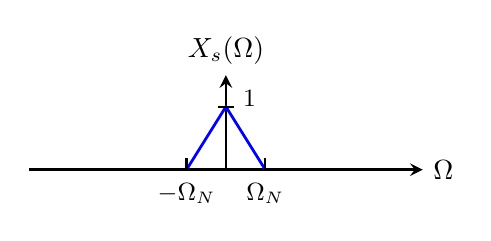
\begin{tikzpicture}
        \centering 
        % Set up styles
        \tikzset{line style/.style={thick}}
        % Frequency axis
        \draw[-stealth, line width=1pt] (-2.5, 0) -- (2.5, 0) node[right] {$\Omega$};
        \draw[-stealth, line width=1pt] (0, 0) -- (0, 1.2) node[above] {$X_{s}(\Omega)$};
        % Draw and label the triangles
        \draw[line style, line width=1pt, blue] (-0.5, 0) -- (0, 0.8) -- (0.5, 0);
        \draw[line style] (0, 0) -- (0, 0.15);
        \draw[line style] (0.5, 0) -- (0.5, 0.15);
        \draw[line style] (-0.5, 0) -- (-0.5, 0.15);
        % Label the frequency points
        \node at (0.5, -0.3) {\small$\Omega_N$};
        \node at (-0.5, -0.3) {\small$-\Omega_N$};
        % peak value
        \draw[line style] (-0.1, 0.8) -- (0.1, 0.8);
        \node at (0.3, 0.9) {\small 1};
    \end{tikzpicture}
    \hspace{.1\textwidth}
    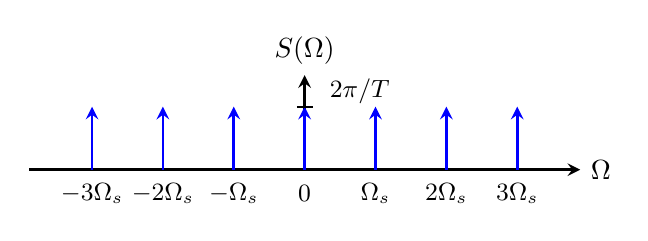
\begin{tikzpicture}
        \tikzset{line style/.style={thick}}
        % Frequency axis
        \draw[-stealth, line width=1pt] (-3.5, 0) -- (3.5, 0) node[right] {$\Omega$};
        \draw[-stealth, line width=1pt] (0, 0) -- (0, 1.2) node[above] {$S(\Omega)$};
        % Draw and label the main triangles and dashed extensions
        \foreach \x in {-2.7, -1.8, -0.9, 0, 0.9, 1.8, 2.7} {
            \draw[line style, -stealth, blue, line width=1pt] (\x, 0) -- (\x, 0.8);
        }
        \node at (-0.9, -0.3) {\small$-\Omega_s$};
        \node at (-1.8, -0.3) {\small$-2\Omega_s$};
        \node at (-2.7, -0.3) {\small$-3\Omega_s$};
        \node at (0, -0.3) {\small 0};
        \node at (0.9, -0.3) {\small$\Omega_s$};
        \node at (1.8, -0.3) {\small$2\Omega_s$};
        \node at (2.7, -0.3) {\small$3\Omega_s$};
        % peak
        \draw[line style] (-0.1, 0.8) -- (0.1, 0.8);
        \node at (0.7, 1) {\small$2\pi/T$};
    \end{tikzpicture}
    \caption{Spectrum of (left) the original continuous-time signal to be sampled, $X_s(\Omega)$ and (right) the sampler $S(\Omega)$ (as a $\delta$-train).}
    \label{fig:original_signal}
\end{figure}

For sampled signals: $\Omega_{N}$ is the signal bandwidth
\begin{itemize}
    \item if $\Omega_{s} \geq 2\Omega_{N}$, the replicas in the periodization do not overlap (\autoref{fig:aliasing}.a)
    \item if $\Omega_{s} < 2\Omega_{N}$, the replicas overlap, also known as \textbf{aliasing}(\autoref{fig:aliasing}.b).
\end{itemize} 

\begin{figure}[H]
%% first figure
\begin{subfigure}{.45\textwidth}
\centering
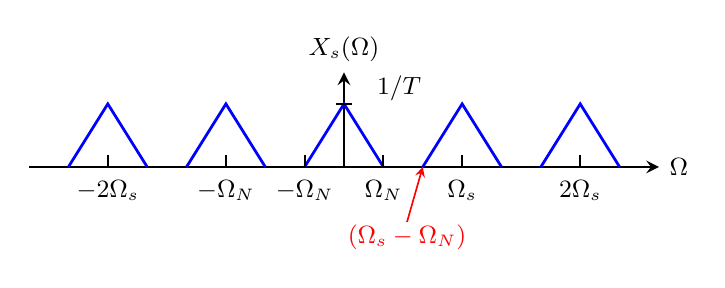
\begin{tikzpicture}
    \tikzset{line style/.style={thick}}
    % frequency axis
    \draw[-stealth, line width=1pt] (-4, 0) -- (4, 0) node[right] {\small$\Omega$};
    \draw[-stealth, line width=1pt] (0, 0) -- (0, 1.2) node[above] {\small $X_{s}(\Omega)$};

    % draw and label the triangles
    \foreach \x in {-3, -1.5, 0, 1.5, 3} {
        \draw[line style, line width=1pt, blue] (\x-0.5, 0) -- (\x, 0.8) -- (\x+0.5, 0);
        \draw[line style] (\x, 0) -- (\x, 0.15);
    }
    \draw[line style] (0.5, 0) -- (0.5, 0.15);
    \draw[line style] (-0.5, 0) -- (-0.5, 0.15);
    
    % label the frequency points
    \node at (0.5, -0.3) {\small$\Omega_N$};
    \node at (-0.5, -0.3) {\small$-\Omega_N$};
    \node at (1.5, -0.3) {\small$\Omega_s$};
    \node at (-1.5, -0.3) {\small$-\Omega_N$};
    \node at (3, -0.3) {\small$2\Omega_s$};
    \node at (-3, -0.3) {\small$-2\Omega_s$};

    % peak value
    \draw[line style] (-0.1, 0.8) -- (0.1, 0.8);
    \node at (0.7, 1) {\small$1/T$};

    % x values below the triangles
    \node[red] at (0.8, -0.9) {\small$(\Omega_s - \Omega_N)$};
    \draw[-stealth, red, line width=.6pt] (0.8, -0.7) -- (1, 0);
\end{tikzpicture}
\caption{Sampling without aliasing when $\Omega_{s} \geq 2\Omega_{N}$.}
\end{subfigure}
\hfill
%% second figure
\begin{subfigure}{.45\textwidth}
\centering
    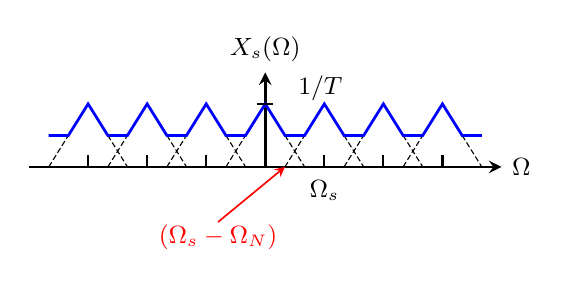
\begin{tikzpicture}
    \tikzset{line style/.style={thick}}
    \tikzset{dashed style/.style={thick, dashed}}

    % Frequency axis
    \draw[-stealth, line width=1pt] (-3, 0) -- (3, 0) node[right] {\small $\Omega$};
    \draw[-stealth, line width=1pt] (0, 0) -- (0, 1.2) node[above] {\small $X_{s}(\Omega)$};

    % Draw and label the main triangles and dashed extensions
    \foreach \x in {-2.25, -1.5, -0.75, 0, 0.75, 1.5, 2.25} {
        \draw[dash pattern=on 2pt off 1pt] (\x-0.5, 0) -- (\x-0.25, 0.4) ;
        \draw[dash pattern=on 2pt off 1pt] (\x+0.25, 0.4) -- (\x+0.5, 0) ;
        \draw[line style, line width=1pt, blue]  (\x-0.5, 0.4) -- (\x-0.25, 0.4) -- (\x, 0.8) -- (\x+0.25, 0.4) -- (\x+0.5, 0.4);
        \draw[line style] (\x, 0) -- (\x, 0.15);
    }
    \node at (0.75, -0.3) {\small$\Omega_s$};

    % peak
    \draw[line style] (-0.1, 0.8) -- (0.1, 0.8);
    \node at (0.7, 1) {\small$1/T$};
    % \node at (0.3, 1.9) {$X_s(\omega)$};

    % x values below the triangles
    \node[red] at (-0.6, -0.9) {\small$(\Omega_s - \Omega_N)$};
    \draw[-stealth, red, line width=.6pt] (-0.6, -0.7) -- (0.25, 0);
\end{tikzpicture}
\caption{Sampling with aliasing when $\Omega_{s} < 2\Omega_{N}$}
\end{subfigure}
\caption{The signal copies remain separate under a high sampling rate; while the signals are overlapped (aliasing) with a lower sampling rate.} 
\label{fig:aliasing}
\end{figure}



\subsubsection{Nyquist-Shannon Sampling Theorem}
Nyquist-Shannon sampling theorem states that: \textbf{to retain the ability to reproduce (reconstruct) the original signal, the minimum sampling frequency during signal sampling must be at least twice its frequency.}\\

Mathematically, let $x_{c}(t)$ be a band-limited signal with $X_{c}(\Omega)=0$, for $\lvert \Omega \rvert \geq \Omega_{N}$. Then $x_{c}(t)$ is uniquely determined by its samples $x[n] = x_{c}(nT)$, if 
\[ \Omega_{s}=\frac{2\pi}{T} \geq 2\Omega_{N} \]
where $2\Omega_{N}$ is the minimal sampling rate and referred to as the \textbf{Nyquist rate}.\\

Nyquist-Shannon sampling theorem provides the condition under which the C/D transformation \textbf{can be inverted} without losing information, as shown in \autoref{fig:nyquist}.

\begin{figure}[H]
    \centering
    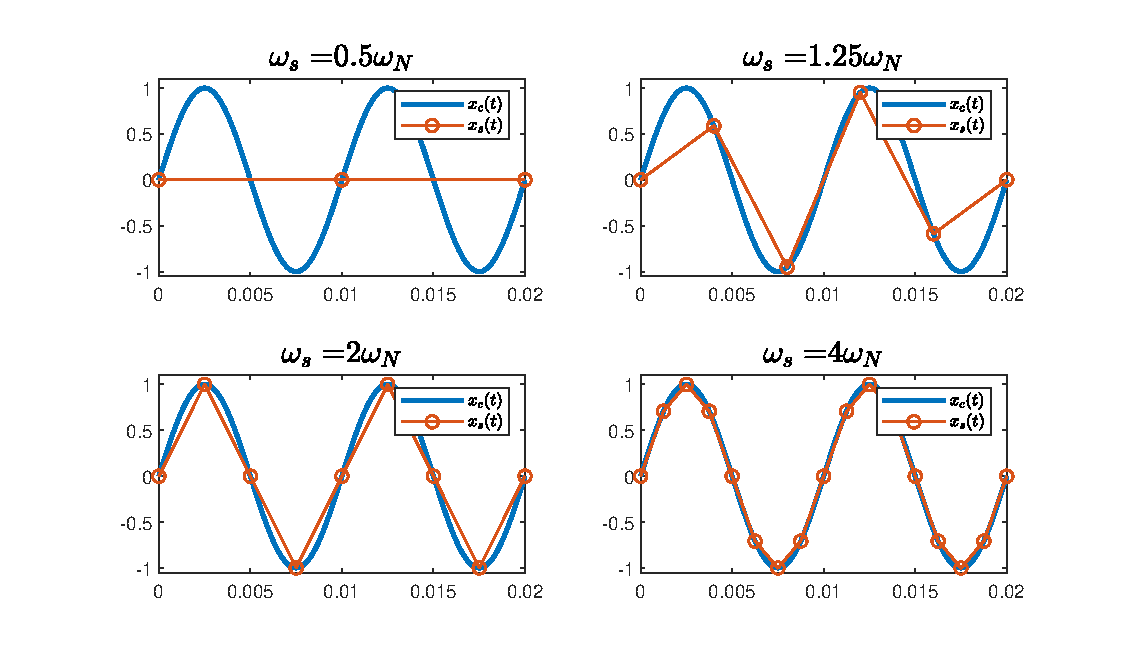
\includegraphics[width=\textwidth, center]{images/nyquist.eps}
    \caption{Sampling of a continuous signal $x_{c}(t)=\sin(200\pi t)$: (left to right, top to bottom) $\Omega_{s}=0.5\Omega_{N}$, $\Omega_{s}=1.25\Omega_{N}$, $\Omega_{s}=2\Omega_{N}$, $\Omega_{s}=4\Omega_{N}$. According to the Nyquist-Shannon sampling theorem, aliasing occurs when $\Omega_{s} < 2\Omega_{N}$}
    \label{fig:nyquist}
\end{figure}

\subsection{Practical Digital Processing of Continuous-Time Signals}
\begin{figure}[H]
    \centering
    \resizebox{\textwidth}{!}{
    \begin{tikzpicture}[auto, node distance=1cm,>=Latex]
        % Nodes
        % 1
        \node (input) {$x_c(t)$};
        \node [draw, rectangle, minimum width=2.5cm, minimum height=1cm, right=.7cm of input] (block1) {\parbox{2.5cm}{\centering \textbf{anti-aliasing filter}}};
        \node[above=.15cm of block1]{$H_{aa}(j\Omega)$};
        \node [right=.45cm of block1] (xat) {};
        \node [below=0.05cm of xat] (xat_label) {$x_{a} (t)$};
        % 2
        \node [draw, rectangle, minimum width=2cm, minimum height=1cm, right=.45cm of xat] (block2) {\parbox{2cm}{\centering \textbf{sample and hold}}};
        \node [right=.45cm of block2] (x0t) {};
        \node [below=0.05cm of x0t] (x0t_label) {$x_{0}(t)$};
        % 3
        \node [draw, rectangle, minimum width=2cm, minimum height=1cm, right=.45cm of x0t] (block3) {\parbox{2cm}{\centering \textbf{A/D converter}}};
        \node [right=.45cm of block3] (xhatn) {};
        \node [below=0.05cm of xhatn] (xhatn_label) {$\hat{x}[n]$};
        % 4
        \node [draw, rectangle, minimum width=2.5cm, minimum height=1cm, right=.45cm of xhatn] (block4) {\parbox{2.5cm}{\centering \textbf{discrete-time system}}};
        \node [right=.45cm of block4] (yhatn) {};
        \node [below=0.05cm of yhatn] (yhatn_label) {$\hat{y}[n]$};
        % 5
        \node [draw, rectangle, minimum width=2cm, minimum height=1cm, right=.45cm of yhatn] (block5) {\parbox{2cm}{\centering \textbf{D/A converter}}};
        \node [right=.45cm of block5] (yDA) {};
        \node [below=0.05cm of yDA] (yDA_label) {$y_{DA}(t)$};
        % 6
        \node [draw, rectangle, minimum width=2.7cm, minimum height=1cm, right=.45cm of yDA] (block6) {\parbox{2.7cm}{\centering \textbf{reconstruction filter}}};
        \node[above=.15cm of block6]{$\widetilde{H}_{r}(j\Omega)$};
        \node [right=0.7cm of block6] (output) {$\hat{y}_{r}(t)$};
        % T symbs
        \node[below=0.5cm of block2](T2){$T$};
        \node[below=0.5cm of block3](T3){$T$};
        \node[below=0.5cm of block5](T5){$T$};
        
        % Arrows
        \draw[->] (input) -- (block1);
        \draw[->] (block1) -- (block2);
        \draw[->] (block2) -- (block3);
        \draw[->] (block3) -- (block4);
        \draw[->] (block4) -- (block5);
        \draw[->] (block5) -- (block6);
        \draw[->] (block6) -- (output);
        \draw[->] (T2) -- (block2);
        \draw[->] (T3) -- (block3);
        \draw[->] (T5) -- (block5);
    \end{tikzpicture}
    }
    \caption{Overview of practical digital processing of continuous-time signals}
    \label{fig:dsp}
\end{figure}

\paragraph{Ideal anti-aliasing filter: $x_{c}(t) \to x_{a}(t)$} remove all frequencies in time-continuous signal that are above half the sampling rate.
\[
    H_{aa}(j\Omega) = 
    \begin{cases}
    1,  & \lvert \Omega \rvert \leq \pi/T \\
    0,  & \lvert \Omega \rvert > \pi/T
    \end{cases}
\]

\paragraph{Sample and hold: $x_{a}(t) \to x_{0}(t)$}
\[
    x_0(t) = h_0(t) * \sum_{n=-\infty}^{\infty} x_{c}(nT)\delta(t-nT)
\]

\paragraph{Quantization:} the A/D is seen as an integration of a quantizer and a coder. A quantizer is a non-linear system that represents the 
amplitude values of the signal into a finite set of values. \\

In a uniform quantizer, sample values are rounded to the nearest quantization level, followed by binary 
coding.

\paragraph{Practical D/A conversion: $\hat{y}[n] \to y_{DA}(t)$}
\[
    x_{c}(t) = \sum_{n=-\infty}^{+\infty} x_{c}(nT)h_{r}(t-nT) = \sum_{n=-\infty}^{+\infty} x_{c}(nT) \frac{\sin(\pi(t-nT)/T)}{\pi(t-nT)/T}
\]
\[
    x_{DA}(t) = \sum_{n=-\infty}^{+\infty} x[n]h_{p}(t-nT) + \sum_{n=-\infty}^{+\infty} e[n]h_{p}(t-nT)
\]

\subsection{Example Questions}
\begin{q}{}
The continuous-time signal $x_{c}(t)$ is sampled with sampling frequency $\Omega_{s}$ to obtain the sampled signal $x_{s}(t) = x_{c}(t) \sum_{-\infty}^{+\infty} \delta(t-nT)$ with $T$ being the sampling interval ($\Omega_s = \frac{2\pi}{T}$). The Fourier transform of $x_{c}(t)$ is $X_{c}(j\Omega) = \frac{1}{\Omega_{N}} \lvert \Omega \rvert + 1$ for $\lvert \Omega \rvert \leq \Omega_N$ and $X_{c}(j\Omega) = 0$ for $\lvert \Omega \rvert > \Omega_N$. Assuming $\Omega_{s} = \Omega_{N}$, which of the following expressions for the sampled signal $x_{s}(t)$ is correct? 

\begin{enumerate}[label=(\alph*)]
    \item $x_{s}(t) = x_{c}(t)$
    \item $x_{s}(t) = \frac{1}{T}\delta(t)$
    \item $x_{s}(t) = \sum_{-\infty}^{+\infty} \delta(t-nT)$
    \item $x_{s}(t) = 0$
    \item $x_{s}(t) = \sum_{-\infty}^{+\infty} x_{c}(t-nT)$
\end{enumerate}

\begin{flushright}
\begin{blueenv}
    ANS: (d)
\end{blueenv}
\end{flushright}

\end{q}
%==============================================%



\newpage
\section{Discrete-Time Signals and Systems}
\subsection{Discrete-Time Signals}
A discrete-time signal is mathematically represented
as a sequence of data. The
sequence $x$ contains the numbers indexed by
the discrete-time integer $n$:
\[
    x = \{ x[n] \}, \quad -\infty < n < \infty
\]
Any arbitrary sequence can be expressed as the sum of scaled and delayed impulses:
\[
    x[n] = \sum_{k=-\infty}^{+\infty} x[k] \delta[n-k]
\]
where $\delta[n-k]$ is the shift of the unit impulse sequence $\delta[n]$ (Kronecker delta), defined as
\[
    \delta[n] = 
    \begin{cases}
        0,  & n \neq 0 \\
        1,  & n = 0
    \end{cases}
\]

%==================================
\subsection{Discrete-Time Systems}
\begin{figure}[H]
    \centering
    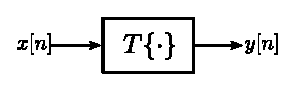
\includegraphics[width=.4\textwidth]{images/discrete-time-system.eps}
    \caption{Representation of a discrete-time system. $T\{\cdot\}$ is a transformation operator that maps an input sequence $x[n]$ into an output sequence $y[n]$.}
    \label{fig:dt_sys}
\end{figure}

\begin{ex}{The Moving Average System}
The moving average system is a discrete-time system. It is defined as
\begin{align*}
    y[n] 
    & = \frac{1}{M_1 + M_2 + 1} \sum_{k=-M_1}^{M_2} x[n-k] \\
    & = \frac{1}{M_1 + M_2 + 1} (x[n+M_1] + x[n+M_1 -1] + ... + x[n] + x[n-1] + x[n-M_2])
\end{align*}
The system computes the $n$\textsuperscript{th} sample of the output sequence as the average of $(M_1+M_2+1)$ samples of the input sequence around the $n$\textsuperscript{th} sample.
\end{ex}
%==================================
\subsubsection{Memoryless Systems}
A system is \textit{memoryless} if the system output $y[n]$ at every value of $n$ depends only on the input $x[n]$ at the same value of $n$.
\begin{ex}{A Memoryless System}
    \[
        y[n] = (x[n])^2, \quad \text{for each value of $n$.}
    \]
\end{ex}
%==================================
\subsubsection{Linear Systems}
A system is \textit{linear} if and only if
\[
    T\{ x_{1}[n] + x_{2}[n] \} 
    =  T\{ x_{1}[n] \} + T\{ x_{2}[n] \}
    = y_{1}[n] + y_{2}[n]
\]
and
\[
     T\{ ax[n] \} = a T\{ x[n] \} = ay[n]
\]

\begin{ex}{The Accumulator System}
The system
    \[
        y[n] = \sum_{k=-\infty}^{n}x[k]
    \]
is an accumulator system as the output at $n$ is the sum of the present and all previous input samples. The system is linear, as the proof shown below: define two arbitrary inputs $x_{1}[n]$ and $x_{2}[n]$ and their corresponding outputs:
\[
    y_{1}[n] = \sum_{k=-\infty}^{n}x_{1}[k]
\]
\[
    y_{2}[n] = \sum_{k=-\infty}^{n}x_{2}[k]
\]
When $x_{3}[k] = ax_{1}[n] + bx_{2}[n]$, 
\begin{align*}
    y_{3}[n]
    & = \sum_{k=-\infty}^{n}x_{3}[k] \\
    & = \sum_{k=-\infty}^{n} (ax_{1}[n] + bx_{2}[n]) \\
    & = a \sum_{k=-\infty}^{n} x_{1}[k] + b \sum_{k=-\infty}^{n} x_{2}[k] \\
    & = ay_{1}[k] + by_{2}[k]
\end{align*}
Therefore, the accumulator system is linear.
\end{ex}
%==================================
\subsubsection{Time-Invariant Systems}
A system is \textit{time-invariant} if the shift or delay of the input sequence causes a corresponding shift in the output sequence. Mathematically, if $y[n] = T\{x[n]\}$, the input sequence $x_{1}[n]=x[n-n_0]$ produces at output the sequence $y_{1}[n]=y[n-n_0]$. 

\begin{ex}{The Compressor System}
A compressor is defined by the relation
\[
    y[n] = x[Mn], \quad -\infty < n \infty
\]
with $M$ a positive integer. The system creates the output sequence by selecting every $M$\textsuperscript{th} sample. \\

This system is \textit{not} time-invariant, as the proof shown below: consider a system output $y_1[n]$ corresponding to the input $x_1[n]=x[n-n_0]$, 
\[
    y_1[n] = x_1[Mn] = x[Mn-n_0]
\]
If the system is time-invariant, the input to the system $x_1[n]$ should yield the output $y[n-n_0]$,
\[
    y[n-n_0] = x[M(n-n_0)]
\]
Clearly, $x[Mn-n_0] \neq x[M(n-n_0)]$ $\to$ the system is not time-invariant. 
\end{ex}
%==================================
\subsubsection{Causality}
A system is \textit{causal} if, for every choice of $n_0$, the output sequence value at the index $n=n_0$ depends only on the input sequence values for $n\leq n_0$, \textit{i.e.}, the system output purely depends on the past and current input, not future input. 

\begin{ex}{The Forward and Backward Difference Systems}
\begin{itemize}
    \item \textbf{The forward difference system} is defined as
    \[
        y[n] = x[n+1] - x[n]
    \]
    Clearly, the forward difference system is \textit{not} causal, since the current value of the output depends on a future value of the input. \underline{Mathematically,} consider two inputs and their outputs:
    \begin{itemize}
        \item $x_1[n]=\delta[n-1] \ \longrightarrow \ y_1[n]=\delta[n]-\delta[n-1], \quad \text{for all $n$}$

        \item $x_2[n]=0 \ \longrightarrow \ y_2[n]=0, \quad \text{for all $n$}$
    \end{itemize}

    Note that $x_1[n] = x_2[n]$ for $n \leq 0$ \footnote{ By definition, $n_0$ can be randomly selected, $n_0=1, 2,...$ also works for this example!}, so by definition of causality, $y_1[n] = y_2[n]$ should always hold for $n \leq 0$, for which the case $n=0$ is an exception that violates the condition for causality - the system is not casual. % counterexample

    \item \textbf{The backward difference system} is defined as
    \[
        y[n] = x[n] - x[n-1]
    \]
    The backward difference system is causal since the output only depends on the present and past values of the input. Same mathematical proof as above.
\end{itemize}
\end{ex}
%==================================
\subsubsection{Stability}
A system is \textit{stable} if and only if every bounded input sequence produces a bounded output sequence (bounded input, bounded output, BIBO). Mathematically, if the input $x[n]$ is bounded, there exists a fixed positive finite value $B_x$ such that 
\[
    \lvert x[n] \rvert \leq B_x < \infty, \quad \text{for all $n$}
\]
and there exists a fixed positive finite value $B_y$ corresponding to every bounded input, 
\[
     \lvert y[n] \rvert \leq B_y < \infty, \quad \text{for all $n$}
\]

\begin{ex}{The Accumulator System (cont'd)}
    The accumulator system is \textit{not} stable: consider the case when $x[n]=u[n]$, the input is bounded by $B_x = 1$. The output 
    \[
        y[n] = \sum_{k=-\infty}^{n}u[k] = 
        \begin{cases}
        0,      & n<0   \\
        (n+1),  & n \geq 0
        \end{cases}
    \]
    Clearly, there is no finite bound $B_y$ such that $(n+1) \leq B_y < \infty$. The system is unstable.
\end{ex}

%% subsection
\subsection{Linear, Time-Invariant (LTI) Systems}

The output of an LTI system is fully determined by the response of the system to the impulse. 
\[
    y[n] 
    = T\{x[n]\}
    = T \bigg\{\sum_{k=-\infty}^{+\infty} x[k] \delta[n-k] \bigg\}
    = \sum_{k=-\infty}^{+\infty} x[k] T \{\delta[n-k]\}
    = \sum_{k=-\infty}^{+\infty} x[k] h[n-k]
\]
where $h[n-k]$ is the system response to the impulse $\delta[n-k]$.\\

The relation between the input and output of an LTI system is expressed by convolution. 
\[
    y[n] = \sum_{k=-\infty}^{+\infty} x[k] h[n-k] = x[n] * h[n]
\]

\begin{ex}{Frequency Response of the Moving Average System}
The impulse response of the moving average system is
\[
    h[n] = 
    \begin{cases}
        \frac{1}{M_1+M_2+1},    & -M_1 \leq n \leq M_2 \\
        0,  & \text{otherwise}
    \end{cases} 
\]
The frequency response with $M_1=0$ is
\begin{align*}
    H(e^{j\omega}) 
    & = \frac{1}{M_2+1} \sum_{n=0}^{M_2}e^{-j\omega n} \\
    & = \frac{1}{M_2+1} \bigg( \frac{1-e^{-j\omega (M_{2}+1)}}{1-e^{-j\omega}} \bigg) \\
    & = \frac{1}{M_2+1} \frac{(e^{j\omega(M_{2}+1)/2} - e^{-j\omega(M_{2}+1)/2})e^{-j\omega(M_{2}+1)/2}}{(e^{j\omega/2}-e^{-j\omega/2})e^{-j\omega/2}} \\
    & = \frac{1}{M_2+1} \frac{\sin[\omega(M_{2}+1)/2]}{\sin \omega/2}e^{-j\omega M_{2}/2}
\end{align*}
\end{ex}

\subsection{Example Exam Question}
%==================================
\begin{q}{}
Consider the linear, time-invariant (LTI) system with impulse response $h[n] = \delta[n] - 2\delta[n-1] + 3\delta[n-2]$. This system is:
\begin{enumerate}[label=(\alph*)]
    \item Non-causal, with memory
    \item Memoryless
    \item Non-causal, stable
    \item Causal, with memory
    \item Unstable
\end{enumerate}
\end{q}
%==================================


\newpage
\section{Discrete-Time and Discrete Fourier Transform}
\subsection{Discrete-Time Fourier Transform}
\begin{itemize}
    \item The discrete-time Fourier transform (DTFT) is defined as
    \[
        X(e^{j\omega}) = \sum_{n=-\infty}^{+\infty} x[n] \ e^{-j\omega n}.
    \]
        

    \item Inverse transform
    \begin{align*}
        x[n]
        &= \frac{1}{2\pi} \int_{-\pi}^{+\pi} X(e^{-j\omega}) e^{j\omega n} \mathrm{d}\omega \\
        &= \lim_{\Delta \omega \to 0} \sum_{k} [X(e^{jk\Delta \omega})\frac{\Delta \omega}{2\pi}]e^{jk\Delta \omega n}
    \end{align*}
    Fourier transform decomposes sequences using a linear combination of complex exponentials with incremental amplitudes.

    \item Therefore, the frequency response of a LTI system is the Fourier transform of the impulse response:
    \[
        H(e^{j\omega}) = \sum_{n=-\infty}^{+\infty} h[n] e^{-j\omega n}
    \]
\end{itemize}

\begin{ex}{Frequency Response of the Moving Average System}
The impulse response of the moving average system is
\[
    h[n] = 
    \begin{cases}
        \frac{1}{M_1+M_2+1},    & -M_1 \leq n \leq M_2 \\
        0,  & \text{otherwise}
    \end{cases} 
\]
The frequency response with $M_1=0$ is
\begin{align*}
    H(e^{j\omega}) 
    & = \frac{1}{M_2+1} \sum_{n=0}^{M_2}e^{-j\omega n} \\
    & = \frac{1}{M_2+1} \bigg( \frac{1-e^{-j\omega (M_{2}+1)}}{1-e^{-j\omega}} \bigg) \\
    & = \frac{1}{M_2+1} \frac{(e^{j\omega(M_{2}+1)/2} - e^{-j\omega(M_{2}+1)/2})e^{-j\omega(M_{2}+1)/2}}{(e^{j\omega/2}-e^{-j\omega/2})e^{-j\omega/2}} \\
    & = \frac{1}{M_2+1} \frac{\sin[\omega(M_{2}+1)/2]}{\sin \omega/2}e^{-j\omega M_{2}/2}
\end{align*}
\end{ex}

%% subsection
\subsection{Properties of DTFT}

\paragraph{Periodicity}  If $x[n] \ \xleftrightarrow[]{\mathcal{F}} \ X(e^{j\omega})$, then
\[
    X(e^{j\omega}) =  X(e^{j (\omega+2\pi)}),
\]
\textit{i.e.}, $X(e^{j\omega})$ is $2\pi$-periodic.

\paragraph{Linearity} If $x_1[n] \ \xleftrightarrow[]{\mathcal{F}} \ X_1(e^{j\omega})$ and $x_2[n] \ \xleftrightarrow[]{\mathcal{F}} \ X_2(e^{j\omega})$, then 
\[
    a_1 x_1 [n] + a_2 x_2 [n] \ \xleftrightarrow[]{\mathcal{F}} \ a_1 X_1(e^{j\omega}) + a_2 X_2(e^{j\omega}),
\]
where $a_1$ and $a_2$ are arbitrary real-valued or complex-valued constants.

\paragraph{Translation (Time and Frequency Shifting)} If $x[n] \ \xleftrightarrow[]{\mathcal{F}} \ X(e^{j\omega})$, then the time shifting property is
\[
    x[n - n_{d}] \ \xleftrightarrow[]{\mathcal{F}} \ e^{-j\omega n_{d}} X(e^{j\omega}),
\]
where $n_d$ is an arbitrary integer. Similarly, the frequency shifting property is
\[
    e^{j\omega_d n} x[n]\}  \ \xleftrightarrow[]{\mathcal{F}} \ X(e^{j(\omega-\omega_d)})
\]


\paragraph{Conjugate Symmetry} 
For a real-valued sequence $x[n]$, if $x[n] \ \xleftrightarrow[]{\mathcal{F}} \ X(e^{j\omega})$, then
\[
    X(e^{j\omega}) = X^{*}(e^{-j\omega}), 
\]
where the asterisk * denotes the complex conjugate (not convolution here).

\begin{itemize}
    \item The magnitude of DTFT, $\lvert X(e^{j\omega}) \rvert$ is an \textit{even} function of $\omega$.

    \item The magnitude of DTFT, $\angle X(e^{j\omega})$ is an \textit{odd} function of $\omega$.
\end{itemize}

\begin{dv}{}
Fourier transform:
\[
    X(e^{j\omega}) =  \sum_{n=-\infty}^{+\infty} x[n] e^{-j\omega n}
\]
Replace $\omega$ to $-\omega$:
\[
    X(e^{-j\omega}) =  \sum_{n=-\infty}^{+\infty} x[n] e^{+j\omega n}
\]
Take the complex conjugate of the Fourier transform above: 
\[
    X^{*}(e^{-j\omega}) =  \sum_{n=-\infty}^{+\infty} \underbrace{x^{*}[n]}_{x[n]} e^{-j\omega n}
\]
Since $x[n] \in \mathbb{R}$, the complex conjugate of the Fourier transform is equivalent to Fourier transform:
\[
    X(e^{-j\omega}) = X^{*}(e^{-j\omega})
\]
\rule{\textwidth}{.1ex}
Furthermore, express the Fourier transform in terms of a real part and an imaginary part:
\[
    X(e^{j\omega}) = X_{\mathbb{R}}(e^{j\omega}) + j X_{\mathbb{I}}(e^{j\omega})
\]
The complex conjugate of the Fourier transform is thus
\[
    X^{*}(e^{-j\omega}) = X_{\mathbb{R}}(e^{-j\omega}) - j X_{\mathbb{I}}(e^{-j\omega})
\]
Equate the two expressions above, 
\[
    X_{\mathbb{R}}(e^{j\omega}) = X_{\mathbb{R}}(e^{-j\omega})
\]
\[
    X_{\mathbb{I}}(e^{j\omega}) = -X_{\mathbb{I}}(e^{-j\omega})
\]
That's saying, the real part of the Fourier transform is an \textit{even} function of $\omega$, and the imaginary part of the Fourier transform is an \textit{odd} function of $\omega$.
The magnitude of the Fourier transform is an \textit{even} function of $\omega$; the phase of the Fourier transform is an \textit{odd} function of $\omega$.
\end{dv}

\paragraph{Time Reversal} If $x[n] \ \xleftrightarrow[]{\mathcal{F}} \ X(e^{j\omega})$, then
\[
    x[-n] \ \xleftrightarrow[]{\mathcal{F}} \  X(e^{-j\omega}) = X^*(e^{j \omega}).
\]


\paragraph{Parseval's Theorem}
\[
    \sum_{n=-\infty}^{+\infty} \lvert x[n] \rvert^2 =\frac{1}{2\pi} \int_{-\infty}^{+\infty} \lvert X(e^{j\omega}) \rvert^2 \mathrm{d}\omega 
\]
where $\lvert X(e^{j\omega}) \rvert^2$ is the \textit{energy density spectrum} of the sequence, which determines how the energy is distributed in the frequency domain.

\paragraph{Convolution} If $x_1[n] \ \xleftrightarrow[]{\mathcal{F}} \ X_1(e^{j\omega})$ and $x_2[n] \ \xleftrightarrow[]{\mathcal{F}} \ X_2(e^{j\omega})$, then 
\[
    x_1[n] * x_2[n] \ \xleftrightarrow[]{\mathcal{F}} \ X_1(e^{j\omega}) X_2(e^{j\omega}),
\]
\textit{i.e.}, the convolution of two signals in the time domain is equivalent to the multiplication in the frequency domain. That is saying, for an LTI system, we have 
\[
    y[n] = x[n] * h[n] \ \xleftrightarrow[]{\mathcal{F}} \  Y(e^{j\omega}) = X(e^{j\omega})H(e^{j\omega}).
\]
    

%% subsection
\subsection{Common DTFT Pairs}
\begin{table}[H]
    \centering
    \begin{tabular}{c c}
    \toprule
    $x[n]$    & $X(e^{j\omega})$ \\ 
    \midrule
        $\delta[n]$     &   1  \\[.5em]
        
        1   &   $2\pi \sum_{n=-\infty}^{+\infty} \delta(\omega-2\pi n)$ \\[.5em]
        
        $u[n]$  &   $\frac{e^{j\omega}}{e^{j\omega}-1} \sum_{n=-\infty}^{+\infty} \pi \delta(\omega-2\pi n)$ \\[.5em]
        
        $a^n u[n]$, $\lvert a \rvert <1$    &   $\frac{e^{j\omega}}{e^{j\omega}-a}$ \\[.5em]

        $-a^n u[-n-1]$, $\lvert a \rvert >1$    &   $\frac{e^{j\omega}}{e^{j\omega}-a}$ \\[.5em]

        $a^{\lvert n \rvert}$, $\lvert a \rvert <1$     &   $\frac{1-a^2}{1-2a\cos\omega+a^2}$ \\[.5em]

        $\cos(\omega_0 n)$    &   $\pi \sum_{k=\infty}^{+\infty} [\delta(\omega -\omega_0 - 2\pi k) + \delta(\omega +\omega_0 - 2\pi k)]$ \\[.5em]

        $\sin(\omega_0 n)$    &   $j\pi \sum_{k=\infty}^{+\infty} [\delta(\omega + \omega_0 - 2\pi k) - \delta(\omega - \omega_0 - 2\pi k)]$ \\[.5em]

        $u[n] - u[n-M]$ &   $e^{-j\omega(M-1)/2} (\frac{\sin(M\omega/2)}{\sin(\omega/2)})$\\[.5em]
    \bottomrule
    \end{tabular}
\end{table}

%% subsection
\subsection{From DTFT to Discrete Fourier Transform (DFT)}

\paragraph{Sampling the frequency domain in DTFT leads to the DFT}
\begin{itemize}
    \item The discrete-time Fourier transform (DTFT) requires a continuity of its frequency $\omega$.

    \item If we sample the frequency $\displaystyle \omega = \frac{2\pi k}{N}$ where $k \in [0, N-1]$ from DTFT, the sampled signal $X[k]$ is
    \[
        X[k] = X(e^{j\omega})\lvert_{\omega = \frac{2\pi k}{N}} \ = \ \sum_{n=0}^{N-1} x[n] \ e^{-j {\color{red}\frac{2\pi k}{N}} n}.
    \]
    This process is the \textbf{discrete Fourier transform} (DFT). DFT is a sequence with the same duration as the discrete-time sequence, with a sampled frequency axis.

    \item The \textbf{inverse discrete Fourier transform} is
    \[
        x[n] = \frac{1}{N} \sum_{k=0}^{N-1} X[k] \ e^{{j \color{red}\frac{2\pi k}{N}} n}.
    \]
    DFT is sufficient to reconstruct the original discrete-time series, given the discrete-time series is of finite duration.
\end{itemize}

\paragraph{What happens when we sample the frequency domain?} Let $\widetilde{X}(e^{j\omega})$ denote the signal results from sampling $X(e^{j\omega})$ at the frequency $\displaystyle \omega = \frac{2\pi k}{N}$ (where $k \in [0, N-1]$):
\[
    \widetilde{X}(e^{j\omega}) = X(e^{j\omega})  \ \overbrace{\sum_{k=-\infty}^{+\infty} \delta \left(\omega-\frac{2\pi k}{N} \right)}^{\text{\color{gray} sampler}},
\]
by applying the inverse Fourier transform of $\widetilde{X}(e^{j\omega})$,
\[
    \widetilde{x}[n] = N \sum_{k=-\infty}^{+\infty} x[n-kN],
\]
for which we now obtained a periodic signal (in its time domain). This tells us that \textbf{sampling the Fourier transform in the \textit{frequency} domain corresponds to the periodization in the \textit{time} domain}.

\begin{figure}[H]
\centering
\begin{subfigure}{\textwidth}
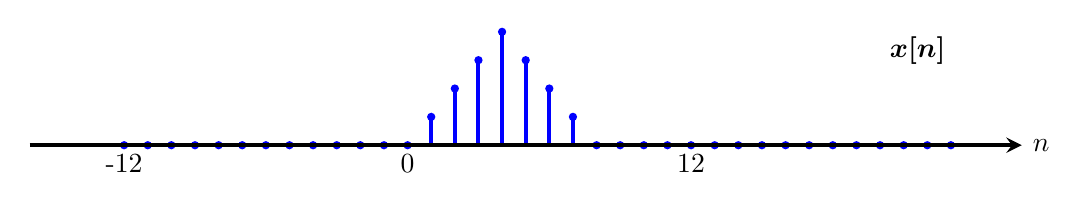
\begin{tikzpicture}[scale = 0.6]
    % Parameters
    \def\N{12} % Period of the signal
    \def\signalLength{8} % Length of the non-zero signal within each period

    % Draw the periodic signal
    \foreach \k in {-1, 0, 1} { % Loop over different periods
        \foreach \n in {0, 1, ..., 11} { % Loop over the entire period
            % Define the height with x = 4 being the highest
            \ifnum\k=0
            \ifnum\n<9
                \pgfmathsetmacro{\height}{0.6*(4 - abs(\n - 4))} % Set non-zero heights for n=0 to n=8
            \else
            \pgfmathsetmacro{\height}{0} % Set height to 0 for n=9 to n=11
            \fi
            \else
                \pgfmathsetmacro{\height}{0} % Set height to 0 for n=9 to n=11
            \fi
            
            \draw[thick, line width=0.5mm, blue] (0.5*\k*\N + 0.5*\n, 0) -- (0.5*\k*\N + 0.5*\n, \height); % Draw vertical line
            \fill[blue] (0.5*\k*\N + 0.5*\n, \height) circle (2.5pt); % Mark the top of the bar
        }
    }
    % Draw the horizontal axis
    \draw[-stealth, line width=.5mm] (-8, 0) -- (13, 0) node[right] {$n$};
    % Add key points and labels
    \foreach \x in {-12, 0, 12} {
        \node[below] at (0.5*\x, 0) {\x};
    }

    \node[right] at (10, 2) {$\displaystyle \boldsymbol{x[n]}$};
\end{tikzpicture}
\caption{Finite sequence of $x[n]$}
\end{subfigure}

\begin{subfigure}{\textwidth}
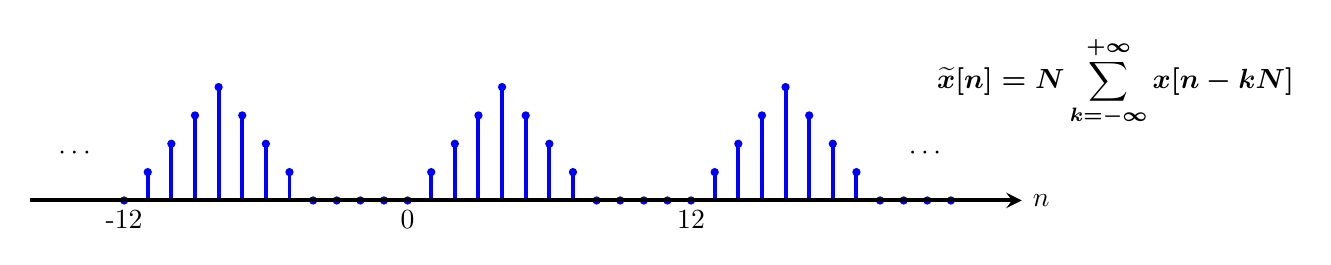
\begin{tikzpicture}[scale=0.6]
    % Parameters
    \def\N{12} % Period of the signal
    \def\signalLength{8} % Length of the non-zero signal within each period

    % Draw the periodic signal
    \foreach \k in {-1, 0, 1} { % Loop over different periods
        \foreach \n in {0, 1, ..., 11} { % Loop over the entire period
            % Define the height with x = 4 being the highest
            \ifnum\n<9
                \pgfmathsetmacro{\height}{0.6*(4 - abs(\n - 4))} % Set non-zero heights for n=0 to n=8
            \else
                \pgfmathsetmacro{\height}{0} % Set height to 0 for n=9 to n=11
            \fi
            
            \draw[thick, line width=0.5mm, blue] (0.5*\k*\N + 0.5*\n, 0) -- (0.5*\k*\N + 0.5*\n, \height); % Draw vertical line
            \fill[blue] (0.5*\k*\N + 0.5*\n, \height) circle (2.5pt); % Mark the top of the bar
        }
    }

    % Draw the horizontal axis
    \draw[-stealth, line width=.5mm] (-8, 0) -- (13, 0) node[right] {$n$};

    % Add key points and labels
    \foreach \x in {-12, 0, 12} {
        \node[below] at (0.5*\x, 0) {\x};
    }
    \node[right] at (11, 2.5) {$\displaystyle \boldsymbol{\widetilde{x}[n] = N \sum_{k=-\infty}^{+\infty} x[n-kN]}$};

    \node at (11, 1) {$\cdots$};
    \node at (-7, 1) {$\cdots$};
\end{tikzpicture}
\caption{Periodic sequence $\widetilde{x}[n]$ corresponding to the sampling of Fourier transform of $x[n]$}
\end{subfigure}
\caption{Illustration of a discrete-time signal $x[n]$ and its periodic extension $\widetilde{x}[n]$.}
\end{figure}

%% subsection
\subsection{Power Spectral Density}
Power spectral density (PSD, also known as the power spectrum) quantifies the power of the signal per unit frequency.
\[
    PSD[k] = \frac{1}{N}\lvert X[k] \rvert^2 = \frac{1}{N} \bigg \lvert  \sum_{n=0}^{N-1} x[n] e^{-j 2 \pi kn/N}\bigg \rvert^2. 
\]

%% subsection
\subsection{Summary}
\begin{figure}[H]
    \centering
    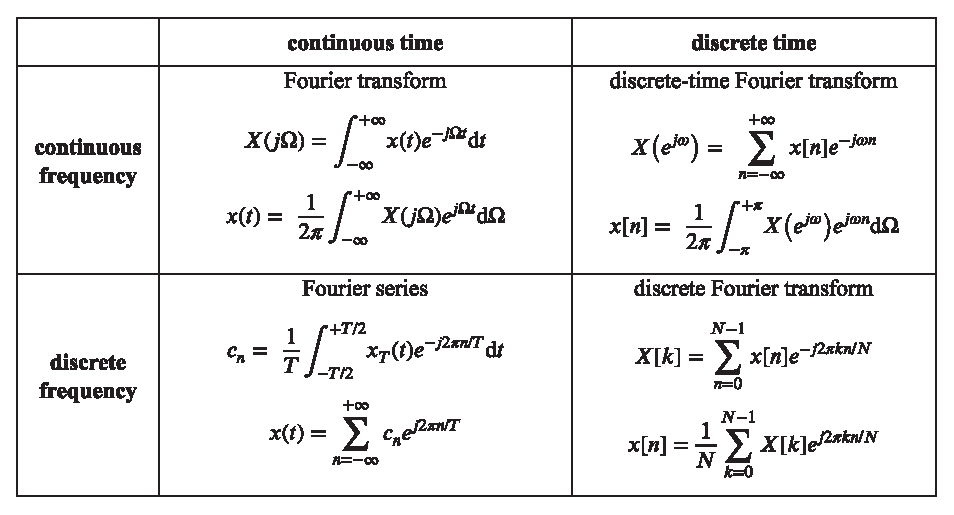
\includegraphics{images/summary_of_FTs.eps}
\end{figure}

\subsection{Example Question}
%==============================================%
\begin{q}{}
Consider the discrete-time signal $x[n] = e^{\frac{j\pi n}{2}}$ and a linear, time-invariant system with transfer function $H(e^{-j\omega}) = e^{-j \omega}$. The output $y[n]$ of this system when the input $x[n]$ is:

\begin{enumerate}[label=(\alph*)]
    \item $y[n] = 0$
    \item $y[n] = -je^{\frac{j\pi n}{2}}$
    \item $y[n] = je^{\frac{j\pi n}{2}}$
    \item $y[n] = x[n] \cdot \lvert H(e^{\frac{j \pi}{2}})\rvert$
    \item $y[n] = x[n]$
\end{enumerate}
\end{q}
%==============================================%
\begin{q}{}
    Given the following discrete-time signal:
    \[
        x[n] = 
        \begin{cases}
            1, & n=0 \\
            -3, & n=1 \\
            -1, & n=2 \\
            0, & n=3
        \end{cases}
    \]
    \begin{enumerate}[label=(\alph*)]
        \item Compute the discrete-time Fourier transform $X(e^{j\omega})$.
        \begin{flushright}
        \begin{blueenv}
            ANS: $X(e^{j\omega}) = 1 - 3e^{-j\omega} - e^{-j2\omega}$.
        \end{blueenv}
        \end{flushright}
        
        \item Compute the discrete Fourier transform $X[k]$ over four points.
        \begin{flushright}
        \begin{blueenv}
            ANS: $X[k] = 
            \begin{cases}
                -3, & k = 0\\
                2+3j, & k = 1\\
                3, & k=2 \\
                2-3j, & k=3
            \end{cases}.$
        \end{blueenv}
        \end{flushright}
        
    \end{enumerate}
    % {\color{blue}
    %     \paragraph{Answer (a)}
    %     \begin{align*}
    %         X(e^{j\omega}) 
    %         & = \sum_{n=0}^{4} x[n] e^{-j\omega n} \\
    %         & = 1 - 3e^{-j\omega} - e^{-j2\omega}
    %     \end{align*}
    % }
    % {\color{blue}
    %     \paragraph{Answer (b)}
    %     \begin{align*}
    %         X[k] 
    %         & = X(e^{j\omega})\lvert_{\omega = \frac{2\pi k}{4}} \\
    %         & = \begin{cases}
    %             -3, & k = 0\\
    %             2+3j, & k = 1\\
    %             3, & k=2 \\
    %             2-3j, & k=3
    %         \end{cases}.
    %     \end{align*}
    % }
\end{q}







\newpage
\section{$z$-transform}
\subsection{$z$-transform}
\paragraph{Definition}
\begin{itemize}
    \item The $z$-transform of a sequence $x[n]$ is:
        \[
            X(z) = \sum_{n=-\infty}^{+\infty} x[n] z^{-n}
        \]
        where $z = re^{j\omega}$ is a complex variable.

    \item Recall that, the discrete-time Fourier transform is defined as
        \[
            X(e^{j\omega}) = \sum_{n=-\infty}^{+\infty} x[n] e^{-j\omega n}
        \]
    Comparing $z$-transform and DTFT, it is clear that the discrete-time Fourier transform is a special case of $z$-transform with $r=1$. Equivalently, $\lvert z \rvert = 1$, as the \textit{unit circle} with $0 \leq \omega \leq 2\pi $ shown in \autoref{fig:z_unit_circ}.
    \begin{figure}[H]
        \centering
        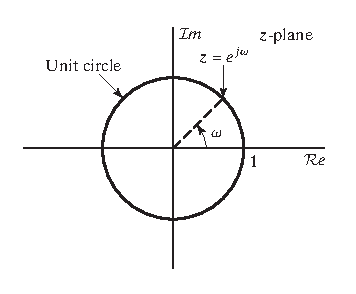
\includegraphics[width=.4\textwidth]{images/z_plane.eps}
        \caption{The unit circle with $r=1$ in the complex $z$-plane}
        \label{fig:z_unit_circ}
    \end{figure}
    This tells us that, the $z$-transform can be viewed as a generalization of the classical Fourier transform.
\end{itemize}

\paragraph{Remarks on the $z$-transform} The $z$-transform is the counterpart of the Laplace transform in the continuous time domain.
\begin{itemize}
    \item Bilateral Laplace transform:
    \[
        X(s) = \int_{-\infty}^{+\infty} x(t) e^{-st} \mathrm{d}t
    \]
    \item $z$-transform:
    \[
        X(z) = \sum_{n=-\infty}^{+\infty} x[n] z^{-n}
    \]
\end{itemize}


\subsection{Region of Convergence}

\begin{itemize}
    \item \textbf{What is the condition for DTFT to converge?} Applying the property \textit{``The magnitude of sum has to be less or equal than the sum of magnitudes"} to the magnitude of Fourier transform (DTFT):
    \begin{align*}
        \lvert X(e^{j \omega}) \rvert
        & = \bigg\lvert \sum_{n=-\infty}^{+\infty} x[n] e^{-j\omega n} \bigg\rvert \leq  \sum_{n=-\infty}^{+\infty} \lvert x[n] \rvert \lvert \cancelto{1}{e^{-j\omega n}} \rvert \\
    \end{align*}
    This conclusion helps us to determine the condition for the convergence of DTFT: if DTFT converges, $\lvert X(e^{j \omega}) \rvert < \infty$, that is
    \[
        \lvert X(e^{j \omega}) \rvert \leq \sum_{n=-\infty}^{+\infty}\lvert x[n] \rvert < \infty
    \]
    we thus only need to evaluate the value of $\sum_{n=-\infty}^{+\infty}\lvert x[n] \rvert$.

    \item \textbf{Not all Fourier transform converges!} The power series representing the Fourier transform does not converge for all sequences, the infinite sum may not always in finite.
    
    \begin{minipage}{.45\textwidth}
    \begin{ex}{}
    For $x[n] = (\frac{1}{2})^n u[n]$, the Fourier transform converges to 2:
    \[
    \sum_{n=-\infty}^{+\infty} \lvert x[n] \rvert = 2
    \]
    \end{ex}
    \end{minipage} \hfill
    \begin{minipage}{.45\textwidth}
    \begin{ex}{}
    For $x[n] = (2)^n u[n]$, the Fourier transform diverges:
    \[
    \sum_{n=-\infty}^{+\infty} \lvert x[n] \rvert = +\infty
    \]
    \end{ex}
    \end{minipage}

    \item Extending the aforementioned concept to the $z$-transform: $z$-transform does not converge for all values of $z$. For any given sequence, the region of values of $z$ for which the $z$-transform power series converges is called the \textit{region of convergence}, or \textit{ROC}.
    \[
        \lvert X(z) \rvert = \bigg\lvert  \sum_{n=-\infty}^{+\infty} x[n] z^{-n} \bigg\rvert \leq \sum_{n=-\infty}^{+\infty} \lvert x[n] \rvert \lvert z \rvert^{-n} < \infty
    \]
    we only need to evaluate the value of $\sum_{n=-\infty}^{+\infty} \lvert x[n] \rvert \lvert z \rvert^{-n}$.

    \item If the convergence condition is satisfied by an arbitrary value $z_1$, then the convergence condition is also satisfies by all values of $z$ such that $\lvert z \rvert = z_1$. Therefore, we can graphically represent the ROC for $0 \leq z_1 < \lvert z \rvert < z_2 \leq \infty$, as shown in \autoref{fig:roc}.
    
    \begin{figure}[H]
        \centering
        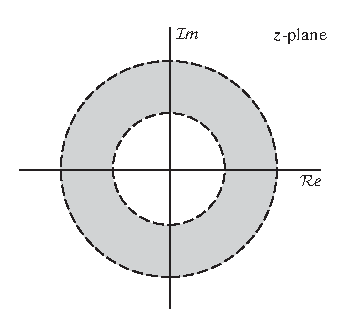
\includegraphics{images/region_of_conv.eps}
        \caption{Graphical representation of region of convergence for $0 \leq z_1 < \lvert z \rvert < z_2 \leq \infty$}
        \label{fig:roc}
    \end{figure}
\end{itemize}

\begin{ex}{ \ Sum of two exponential sequences}
    Consider a signal that is the sum of two real exponentials:
    \[
    x[n] = \bigg( \frac{1}{2} \bigg)^{n} u[n] + \bigg( -\frac{1}{3} \bigg)^{n} u[n]
    \]
    The $z$-transform is 
    \begin{align*}
        X(z) 
        & = \sum_{n=-\infty}^{+\infty} \bigg\{ \bigg( \frac{1}{2} \bigg)^{n} u[n] + \bigg( -\frac{1}{3} \bigg)^{n} u[n] \bigg\} z^{-n} \\
        & = \sum_{n=-\infty}^{+\infty} \bigg( \frac{1}{2} \bigg)^{n} u[n] z^{-n} +  \sum_{n=-\infty}^{+\infty}\bigg( -\frac{1}{3} \bigg)^{n} u[n] z^{-n} \\
        & = \sum_{n=0}^{+\infty} \bigg( \frac{1}{2} z^{-1} \bigg)^{n} +  \sum_{n=0}^{+\infty} \bigg( -\frac{1}{3} z^{-1} \bigg)^{n} \\
        & = \frac{1}{1-\frac{1}{2}z^{-1}} + \frac{1}{1+\frac{1}{3}z^{-1}} = \frac{2(1-\frac{1}{12}z^{-1})}{(1-\frac{1}{2}z^{-1})(1+\frac{1}{3}z^{-1})} \\
        & = \boxed{\frac{2z(z-\frac{1}{12})}{(z-\frac{1}{2})(z+\frac{1}{3})}}
    \end{align*}
    Poles: $z=\frac{1}{2}$, $z=-\frac{1}{3}$, zero: $z=\frac{1}{12}$. For convergence of $X(z)$, it requires both $\displaystyle \bigg\lvert (\frac{1}{2})z^{-1}\bigg\rvert < 1$ and $\displaystyle \bigg\lvert (-\frac{1}{3})z^{-1}\bigg\rvert < 1$. Equivalently, $\lvert z \rvert >\frac{1}{2}$ and $\lvert z \rvert >\frac{1}{3}$. The corresponding pole-zero plot and ROC is shown in \autoref{fig:ex3-3}.
    \begin{figure}[H]
        \centering
        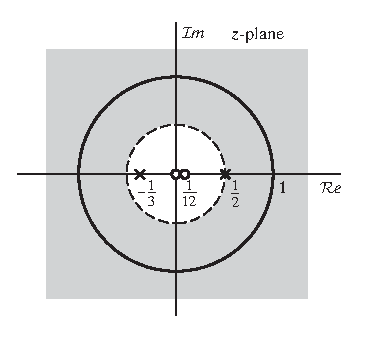
\includegraphics{images/example3-3.eps}
        \caption{Pole-zero plot and ROC for $\frac{2z(z-\frac{1}{12})}{(z-\frac{1}{2})(z+\frac{1}{3})}$}
        \label{fig:ex3-3}
    \end{figure}

    \paragraph{Remarks}
    \begin{itemize}
        \item[-] Sum of geometric sequence: $\displaystyle S_{n} = \frac{a_{1}(r_n - 1)}{r-1}$, where $a_1$ is the first term of the sequence, $r$ is the common ratio. This explains how we get the sum of exponentials above.

        \item[-] One good way to understand the convergence criterion of $X(z)$, we can think the denominator should be negative (\textit{analogous to the stability criterion for a system from Year-2 Control module}).  
    \end{itemize}
\end{ex}

\begin{ex}{ \ Finite-length truncated exponential sequence}
    Consider the signal 
    \[
    x[n] = 
    \begin{cases}
        a^n,    & 0 \leq n \leq N-1, \\
        0,      & \text{otherwise}.
    \end{cases}
    \]
    The $z$-transform is 
    \[
    X(z) = \sum_{n=0}^{N-1} a^{n}z^{-n} = \sum_{n=0}^{N-1} (az^{-1})^n = \frac{1-(az^{-1})^N}{1-az^{-1}} = \boxed{\frac{1}{z^{N-1}} \frac{z^N - a^N}{z-a}}
    \]
    The ROC is determined by the set of $z$ values for which
    \[
    \sum_{n=0}^{N-1} \lvert az^{-1} \rvert^{n} < \infty
    \]
    The sum is finite as long as $az^{-1}$ is finite, which in turn requires only $\lvert a \rvert < \infty$ and $z \neq 0$, leading to the ROC spanning over the entire $z$-plane with an exception of the origin ($z=0$). \\

    For example, with $N=16$ and $0<a<1$, the pole-zero plot is shown in \autoref{fig:ex3-6}.
    \begin{figure}[H]
        \centering
        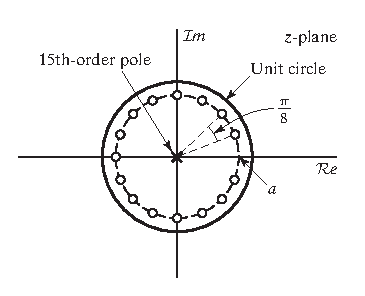
\includegraphics{images/example3-6.eps}
        \caption{Pole-zero plot with $N=16$}
        \label{fig:ex3-6}
    \end{figure}
    Specifically, the $N$ roots of the numerator polynomial are at the $z$-plane locations
    \[
    z_{k} = ae^{j(2\pi k/N)}, \quad k=0, 1, ..., N-1
    \]
\end{ex}

\subsection{Common $z$-Transform Pairs}
\begin{table}[H]
    \centering
    \begin{tabular}{c c c}
    \toprule
    \textbf{Sequence}    & \textbf{Transform}     & \textbf{ROC} \\ 
    \midrule
        $\delta[n]$     &   1   & all $z$  \\[.5em]
        
        $u[n]$     &   $\frac{1}{1-z^{-1}}$   & $\lvert z \rvert >1$  \\[.5em]
        
        $-u[-n-1]$     &   $\frac{1}{1-z^{-1}}$   &  $\lvert z \rvert <1$  \\[.5em]
        
        $\delta[n-m]$     &   $z^{-m}$   & all $z$ except 0 (if $m>0$) or $\infty$ (if $m<0$) \\[.5em]
        
        $a^{n}u[n]$     &  $\frac{1}{1-az^{-1}}$    & $\lvert z \rvert > \lvert a \rvert$\\[.5em]
        
        $-a^{n}u[-n-1]$     &  $\frac{1}{1-az^{-1}}$    & $\lvert z \rvert < \lvert a \rvert$\\[.5em]
        
        $na^{n}u[n]$     &  $\frac{az^{-1}}{(1-az^{-1})^2}$    & $\lvert z \rvert > \lvert a \rvert$\\[.5em]
        
        $-na^{n}u[-n-1]$     &  $\frac{az^{-1}}{(1-az^{-1})^2}$    & $\lvert z \rvert < \lvert a \rvert$\\[.5em]
        
        $\cos(\omega_0 n)u[n]$     &  $\frac{1-\cos(\omega_0)z^{-1}}{1-2\cos(\omega_0)\^{-1}+z^{-2}}$    & $\lvert z \rvert > 1$\\[.5em]

        $\sin(\omega_0 n)u[n]$     &  $\frac{\sin(\omega_0)z^{-1}}{1-2\cos(\omega_0)\^{-1}+z^{-2}}$    & $\lvert z \rvert > 1$\\[.5em]

        $x[n] = 
    \begin{cases}
        a^n,    & 0 \leq n \leq N-1, \\
        0,      & \text{otherwise}.
    \end{cases}$    & $\frac{1-(az^{-1})^N}{1-az^{-1}}$     & $\lvert z \rvert > 0$ \\

    \bottomrule
    \end{tabular}
\end{table}

\subsection{Properties of the $z$-transform}
For the following properties, assume
\[
    x[n] \ \xleftrightarrow[]{\mathcal{Z}} \ X(z)  \quad \quad   ROC = R_x
\]
\[
    x_1[n] \ \xleftrightarrow[]{\mathcal{Z}} \ X_1(z)  \quad \quad   ROC = R_{x1}
\]
\[
    x_2[n] \ \xleftrightarrow[]{\mathcal{Z}} \ X_2(z)  \quad \quad   ROC = R_{x2}
\]
\begin{table}[H]
    \centering
    \begin{tabularx}{\textwidth}{X c c}
    \toprule
    \textbf{Property}    & \textbf{Transform}     & \textbf{ROC} \\ 
    \midrule
        Linearity     &   $ax_1[n]+nx_2[n] \ \xleftrightarrow[]{\mathcal{Z}} \ aX_1(z)+bX_2(z)$   & all $R_{x1} \cap R_{x2}$  \\[.5em]
        
        Time shifting     &   $x[n-n_0] \ \xleftrightarrow[]{\mathcal{Z}} \ z^{-n_0} X(z)$   & $R_{x} (\text{except at $z=0$ and $z=\infty$})$  \\[.5em]
        
        Multiplication by an exponential sequence     &   $z_{0}^{n} x[n] \ \xleftrightarrow[]{\mathcal{Z}} \ X(z/z_0)$   &  $z_0R_x (\lvert z_0 \rvert \lvert z_1 \rvert < \lvert z \rvert < \lvert z_0 \rvert \lvert z_2 \rvert)$  \\[.5em]
        
        Differentiation     &   $nx[n] \ \xleftrightarrow[]{\mathcal{Z}} \ -z \frac{dX(z)}{dz}$   & $R_{x}$ \\[.5em]
        
        Conjugation     &  $ x^{*}[n] \ \xleftrightarrow[]{\mathcal{Z}} \ X^{*}(z^{*})$    & $R_{x}$\\[.5em]
        
        Time reversal    &  $x^{*}[-n] \ \xleftrightarrow[]{\mathcal{Z}} \ X^{*}(1/z^{*})$    & $\frac{1}{R_x} (1/\lvert z_2 \rvert < \lvert z \rvert < 1/\lvert z_1 \rvert)$\\[.5em]

        Convolution    &  $x_1[n] * x_2[n] \ \xleftrightarrow[]{\mathcal{Z}} \ X_{1}(z) X_{2}(z)$    & $R_{x1} \cap R_{x2}$\\[.5em]
        
    \bottomrule
    \end{tabularx}
\end{table}


\begin{ex}{}
Given that 
\[
    x_1[n] = \delta[n] + 2\delta[n-1] + \delta[n-2]
\]
\[
    x_2[n] = \delta[n] -\delta[n-1]
\]
The $z$-transforms of these two sequences are
\[
    X_1(z) = 1 + 2z^{-1} +z^{-2}
\]
\[
    X_2(z) = 1 - z^{-1}
\]
Therefore, if $y[n] = x_{1}[n] * x_{2}[n]$, then
\[
    Y(z) = X_{1}(z)X_{2}(z) = (1 + 2z^{-1} +z^{-2})(1 - z^{-1}) = 1 + z^{-1} - z^{-2} - z^{-3}
\]
\[\Updownarrow\mathcal{Z}^{-1}\]
\[
    y[n] = \delta[n] + \delta[n-1] - \delta[n-2] - \delta[n-3]
\]
\end{ex}


\subsection{LTI Systems and $z$-Transform}
\begin{itemize}
    \item An LTI system is fully characterised by its impulse response. The output $y[n]$ obtained from the input $x[n]$ is:
    \[
    y[n] = x[n] * h[n]
    \]

    \item From the convolution property of the $z$-transform
    \[
    Y(z) = H(z)X(z) 
    \]
    where $H(z) := \mathcal{Z}\{h[n]\}$ is known as the \textbf{system function} of an LTI system.
\end{itemize}

\subsection{Example Questions}
%==============================================%
\begin{q}{}
The $z$-transform of the discrete-time signal $x[n]$ converges for $\lvert a \rvert \leq \lvert z \rvert \leq \lvert b \rvert$, with $0 < \lvert a \rvert \leq \lvert b \rvert$. Which of the following statements is always correct?

\begin{enumerate}[label=(\alph*)]
    \item The discrete-time Fourier transform of $x[n]$ does not converge
    \item The discrete-time Fourier transform of $x[n]$ converges
    \item The discrete-time Fourier transform of $x[n]$ converges if $1 < \lvert a \rvert < \lvert b \rvert$
    \item The discrete-time Fourier transform of $x[n]$ converges if $\lvert a \rvert \leq 1$ and $\lvert b \rvert \geq 1$
    \item The discrete-time Fourier transform of $x[n]$ converges if $\lvert a \rvert < \lvert b \rvert < 1$
\end{enumerate}
\end{q}
%==============================================%
\begin{q}{}
Consider a linear, time-invariant (LTI) system defined by the following difference equation:
\[
    y[n] + \alpha y[n-1] = x[n]
\]
where $\alpha$ is a real number. Which of the following statements is correct?

\begin{enumerate}[label=(\alph*)]
    \item The system is casual and stable for all values of $\alpha$
    \item The system does not have poles for all values of $\alpha$
    \item The system is not causal
    \item The system has a pole for $z=-\alpha$
    \item The system has a pole for $z=\alpha$
\end{enumerate}
\end{q}
%==============================================%
\begin{q}{}
Consider the discrete-time signals $x[n] = a^{-n}u[n-1]$ (where $u[n]$ is the unit step signal and $a$ is a real and positive number different from zero). Which of the following expressions for the $z$-transform of $x[n]$ and its region of convergence (ROC) is correct?

\begin{enumerate}[label=(\alph*)]
    \item $X(z) = \frac{1}{az-1}$ with ROC $\lvert z \rvert > \frac{1}{a}$
    \item $X(z) = \frac{1}{z-a}$ with ROC $\lvert z \rvert > a$
    \item $X(z) = \frac{1}{z+a}$ with ROC $\lvert z \rvert < \frac{1}{a}$
    \item $X(z) = \frac{1}{az-1}$ with ROC $\lvert z \rvert < \frac{1}{a}$
    \item $X(z) = \frac{1}{z-a}$ with ROC $\lvert z \rvert < a$
\end{enumerate}
\begin{flushright}
\begin{blueenv}
    ANS: (a)
\end{blueenv}
\end{flushright}
\end{q}
%==============================================%
\begin{q}{}
Consider the LTI system with the following impulse response $h[n]=\delta[n]-2\delta[n-\dfrac{k}{2}]+\delta[n-k]$, with $k$ an even number.
\begin{enumerate}[label=(\alph*)]
    \item Is the system stable? Is it causal? 
    \begin{flushright}
    \begin{blueenv}
        ANS: stable and casual.
    \end{blueenv}
    \end{flushright}
    
    \item Determine the system function and the transfer function, as a function of $k$.
    \begin{flushright}
    \begin{blueenv}
        ANS: $H(z) = ( 1 - e^{-j\omega \frac{k}{2}} )^2$.
    \end{blueenv}
    \end{flushright}
    
    \item Determine the phase and the group delay of the system, as a function of $k$.
    \begin{flushright}
    \begin{blueenv}
        ANS: $\angle H(e^{j\omega}) = -\frac{k}{2} \omega - \pi$, delayed by $k/2$.
    \end{blueenv}
    \end{flushright}
\end{enumerate}
    
    % {\color{blue}
    % \paragraph{Answer (a)}
    % The system is stable since it has a finite length impulse. The system is causal since for $n<0$, $h[n] = 0$.
    
    % \paragraph{Answer (b)}
    % Compute the $z$-transform of the signal
    % \begin{align*}
    %     h[n] \ & \xleftrightarrow[]{\mathcal{Z}} \ H(z) = 1 - 2z^{-\frac{k}{2}} + z^{-k} \\
    %     & \Rightarrow \ H(e^{j\omega}) = 1 - 2e^{-j\omega \frac{k}{2}} + e^{-j\omega k} = ( 1 - e^{-j\omega \frac{k}{2}} )^2 
    % \end{align*}
    % \color{blue}
    % \paragraph{Answer (c)}
    % From (b), the system function can be re-arranged as
    % \begin{align*}
    %     H(e^{j\omega}) 
    %     &= [e^{-j\omega\frac{k}{4}} (e^{j\omega\frac{k}{4}} - e^{-j\omega\frac{k}{4}})]^2 \\
    %     & = e^{-j\omega\frac{k}{2}} \left[2j\sin \left(\frac{k}{4}\omega \right) \right]^2 \\
    %     & = -4e^{-j\omega\frac{k}{2}} \sin^2 \left(\frac{k}{4}\omega\right) \\
    %     & = +4e^{-j\omega\frac{k}{2}}e^{-j\pi} \sin^2 \left(\frac{k}{4}\omega\right)
    % \end{align*}
    % Hence, the phase of the system is
    % \[
    %     \angle H(e^{j\omega}) = -\frac{k}{2} \omega - \pi,
    % \]
    % with the group delay at $k/2$.
    % }
\end{q}






\newpage
\section{Digital Filters}

\subsection{Filters with Linear Phase}
Recall that a transfer function can be decomposed into the components of the \textbf{magnitude} and \textbf{phase}. For example, an LTI system with the transfer function $H(e^{j\omega}) = e^{-j\omega \alpha}$ with $\lvert \omega \rvert < \pi$ can be expressed as
\[
    H(e^{j\omega}) = \lvert H(e^{j\omega}) \rvert e^{-j\omega \alpha}, \quad \lvert \omega \rvert < \pi,
\]
where $\lvert H(e^{j\omega}) \rvert = 1$ is the magnitude, $\angle H(e^{j\omega}) = -\omega \alpha$ is the phase. 

\paragraph{What does the parameter $\alpha$ do here?} The parameter, $\alpha$, introduces the \textbf{group delay} (or, the time shift) to the input signal in its time domain. This will be more obvious if we further take the inverse Fourier transform of $H(e^{j\omega})$,
\[
    h[n] = \frac{\sin \left (\pi(n-\alpha) \right)}{\pi(n-\alpha)},
\]
where the input signal is delayed by the amount of $\alpha$.

\paragraph{From the perspective of filters...} The transfer function of the form $H(e^{j\omega}) = \lvert H(e^{j\omega}) \rvert e^{-j\omega \alpha}$ tells us that, for an input signal, $x[n]$, the system first \textit{filters} the signal by a zero-frequency response, $\lvert H(e^{j\omega}) \rvert$, following by shirting the filtered signal by $\alpha$. 

\begin{figure}[H]
    \centering
    \begin{tikzpicture}[auto, node distance=2.2cm,>=Latex]
    
        % Nodes
        \node (input) {};
        \node [below=0.05cm of input] (input_label) {$x[n]$};
        \node [draw, rectangle, minimum width=2cm, minimum height=1cm, right=1cm of input] (block1) {$|H(e^{j\omega})|$};
        \node [right=.7cm of block1] (w) {};
        \node [below=0.05cm of w] (w_label) {$w[n]$};
        \node [draw, rectangle, minimum width=2cm, minimum height=1cm, right=1.5cm of block1] (block2) {$e^{-j\omega \alpha}$};
        \node [right=1cm of block2] (output) {};
        \node [below=0.05cm of output] (output_label) {$y[n]$};
    
        % Arrows
        \draw[->] (input) -- (block1);
        \draw[->] (block1) -- (block2);
        \draw[->] (block2) -- (output);
    
        % Labels below arrows
        \node [below=0.1cm of input] {};
        \node [below=0.1cm of w] {};
        \node [below=0.1cm of output] {};
    \end{tikzpicture}
    \caption{Block diagram of a (filter) system with magnitude response $|H(e^{j\omega})|$ followed by phase shift $e^{-j\omega \alpha}$.}
    \label{fig:linear_phase_filter}
\end{figure}

If $\alpha$ is an integer, then the impulse response becomes
\[
    h[n] = \delta[n-\alpha],
\]
the phase of the filter is \textit{linearly proportional} to $\omega$ - we thus say, the filter has a \textbf{linear phase}. \\

We can further generalize the linear-phase systems by extending the phase to be $\angle H(e^{j\omega}) = \beta -\omega \alpha$. Still, if $\alpha$ is an integer, the phase is linearly proportional to $\omega$. The transfer function is
\[
     H(e^{j\omega}) =  A(e^{j\omega})  e^{-j\omega \alpha + j \beta}.
\]


\subsection{Difference Equation}
A \textbf{difference equation} is useful to describe an LTI system. It can be expressed in the following form:
\[
    y[n] = \sum_{k=1}^{N} a_{k}y[n-k] + \sum_{k=0}^{M} b_{k}x[n-k].
\]
\begin{ex}{}
    The LTI system
    \[
        y[n] = x[n] + x[n-1] + ... + x[n-50]
    \]
    is described with a \textit{non-recursive} difference equation.
\end{ex}

\begin{ex}{}
    The LTI system
    \[
        y[n] = y[n-1] + x[n] - x[n-51]
    \]
    is described with a \textit{recursive} difference equation.
\end{ex}

We can find the system function $H(z)$ by taking the $z$-transform for the difference equation:
\begin{align*}
    & y[n] = \sum_{k=1}^{N} a_{k}y[n-k] + \sum_{k=0}^{M} b_{k}x[n-k] \\
    \Rightarrow \quad & y[n] - \sum_{k=1}^{N} a_{k}y[n-k] =  \sum_{k=0}^{M} b_{k}x[n-k] \\
    \xrightarrow[]{\mathcal{Z}} \quad & Y(z) - \sum_{k=1}^{N} a_{k} Y(z) z^{-k} = \sum_{k=0}^{M} b_{k} X(z) z^{-k}\\
    \Rightarrow \quad & H(z) = \frac{Y(z)}{X(z)} = \frac{\sum_{k=0}^{M} b_{k} z^{-k}}{1-\sum_{k=1}^{N} a_{k} z^{-k}} \ {\color{gray} \left( = \frac{B(z)}{A(z)} \right) }
\end{align*}


\subsection{Finite Impulse Response (FIR) Filters}
\subsubsection{Definition}
If $N=0$ in a difference equation, there is no recursive part in $H(z)$ \ (\textit{i.e.}, the output solely depends on the input, the denominator of $H(z)$ is 1, {\color{gray}or $A(z)=1$}),
\[
    H(z) = \sum_{k=0}^{M} b_k \cdot z^{-k}.
\]
This type of filter is known as the \textbf{finite impulse response} (FIR) filter, as illustrated in \autoref{fig:FIR}. \\

\begin{figure}[H]
    \centering
    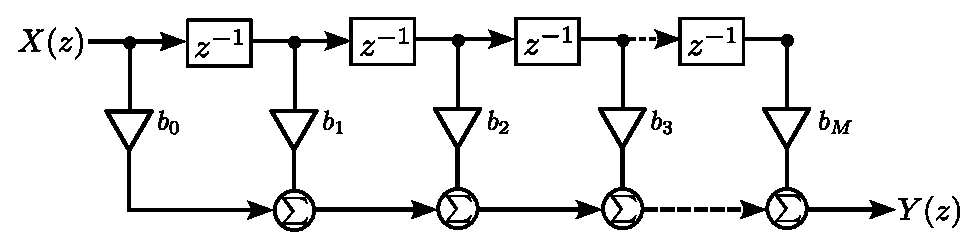
\includegraphics[width=.8\textwidth]{images/FIR_filter.eps}
    \caption{Direct form of a finite impulse response (FIR) filter with linear phase}
    \label{fig:FIR}
\end{figure}


Taking the inverse $z$-transform, we get
\[
    Y(z) = X(z) \underbrace{\sum_{k=0}^{M} b_k \cdot z^{-k}}_{H(z)} \quad \xrightarrow{\mathcal{Z}^{-1}} \quad
    y[n] = \sum_{k=0}^{M} b_k \cdot x[n-k].
\]

\paragraph{Properties of FIR filters}
\begin{itemize}
    \item No poles: all-zero filters. The system function $H(z)$ is defined for the entire $z$-plane.
    \item They are inherently stable. Stability of an LTI system:
    \[
        \sum_{n=-\infty}^{+\infty} \lvert h[n] \rvert < \infty
    \]
    with $h[n]$ of finite length. This condition is always satisfied.
\end{itemize}

\subsubsection{FIR Filter Design by Truncation}
Truncation of the impulse response is a simple way to design FIR filters. Mathematically, we multiply the impulse response with a \textit{window function}.

\begin{ex}{}
The impulse response of an ideal low-pass filter (\autoref{fig:ir_low_pass}) is 
\[
    H(e^{j\omega}) = 
    \begin{cases} 
    1, & \text{if} \ \lvert \omega \rvert \leq \omega_{c} \\ 
    0, & \text{otherwise}
    \end{cases}
    \quad \to \quad
    h_{d}[n] = \frac{\omega_{c}}{\pi}\frac{\sin\omega_{c}n}{\omega_{c}n}
\]
\begin{figure}[H]
    \centering
    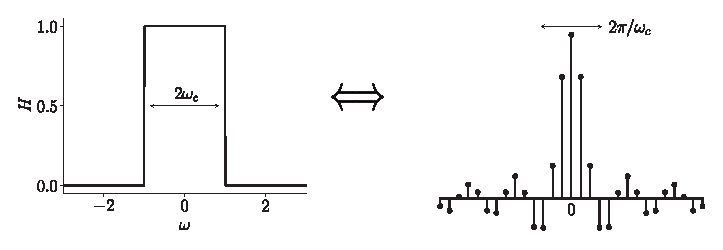
\includegraphics{images/low-pass-response.eps}
    \caption{Impulse response of an ideal low-pass filter}
    \label{fig:ir_low_pass}
\end{figure}

The FIR filter $h[n]$ is created by windowing the ideal response:
\[
    h_{T}[n] = h[n] w[n], \quad \text{for} \ n=0, 1, ..., M
\]
where $w[n]$ is the window function that is only non-zero for $n=0, 1, ..., M$. \autoref{fig:windowing} illustrates the truncation process with a rectangular window function.

\begin{figure}[H]
    \centering
    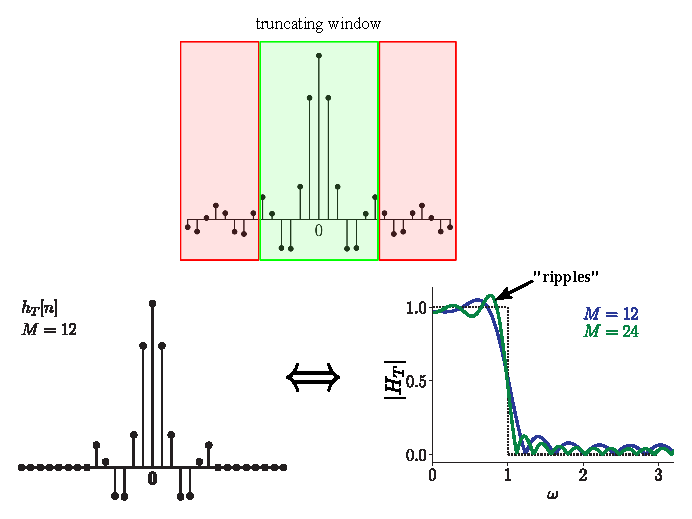
\includegraphics{images/windowing.eps}
    \caption{Truncation of $h[n]$ with a rectangular window.}
    \label{fig:windowing}
\end{figure}

\paragraph{Remarks}
\begin{enumerate}
    \item Typically, the impulse response $h[n]$ is  \textit{non-causal} or at least \textit{non-FIR}. The signal illustrated above is both non-causal and infinite.

    \item Truncation of $h[n]$ to $\pm \frac{M}{2}$ makes the signal finite. Furthermore, the signal will become causal if we delay the truncated signal $h_T[n]$ by $M/2$.

    \item The ripples (indicated with an arrow in \autoref{fig:windowing}) are produced due to the discontinuity of the window \footnote{This can be derived by quantifying the mean squared error in the frequency domain between $H(e^{j\omega})$ and $H_T(e^{j\omega})$. Clearly, the MSE is minimised when $h[n]=h_T[n]$, but practically not possible (regardless of the number of $M$ used in truncation)!}, also referred to as the ``Gibbs phenomenon". 
\end{enumerate}
\end{ex}
From remark (3), although it is impossible to fully remove the ripples, it is possible to truncate with other windows to reduce the ripples. \textit{Hanning}, \textit{Hamming}, \textit{Blackman} (also referred to as \textit{Blackman-Harris}) are examples of alternative windows to rectangular window.

\subsubsection{FIR Filter Design by Other Methods}
\textit{This section is NOT covered in the lectures. Massive materials are adopted from textbooks. Please take prudence with the notations used in this section.}
\begin{itemize}
    \item Frequency sampling: take the IDFT of $M+1$ equally spaced samples of $H(e^{j\omega})$.
    \[
    H_{FIR}(e^{j\omega})=\sum_{n=0}^{M} h[n]e^{-j\omega n} \bigg\lvert_{\omega = \frac{2\pi}{M}k, \quad k=0, 1, 2..., M} \quad \xrightarrow{\mathcal{F}^{-1}} h_{FIR}[n]
    \]
        \begin{itemize}
            \item Pros: giving an exact match at the sample points.
            \item Cons: intermediate approximation is poor if the spectrum varies rapidly.
        \end{itemize}
    \item Least-square
    \item Equiripple method: find the FIR filter to minimise the \textit{maximum weighted error}, $\mathcal{E}$, between the desired response and the actual frequency response of an FIR filter.
    \[
    \mathcal{E}(e^{j\omega}) = \mathcal{W}(\omega)  \lvert H(e^{j\omega}) - H_{FIR}(e^{j\omega})  \rvert
    \]
    where $\mathcal{W}(\omega)$ is a weighting function used to adjust the weightings applied to the pass band, transition band, and stopband:
    \[
    \mathcal{W}(\omega) = \begin{cases}
        1/\delta_1, & 0 \leq \omega \leq \omega_c\\
        0, & \omega_c < \omega < \omega_{s}\\
        1/\delta_2, & \omega_{s} \leq \omega \leq \pi\\
    \end{cases}
    \]
\end{itemize}


\subsection{Infinite Impulse Response (IIR) Filters}

\subsubsection{Definition}
If $N \neq 0$ in the generalized difference equation, the system function carries a recursive part in the denominator. 
\[
    H(z) = \frac{\sum_{k=0}^{M} b_{k} \cdot z^{-k}}{1 - \sum_{k=1}^{N} a_{k} \cdot z^{-k}} \quad \xrightarrow{\mathcal{Z}^{-1}} \quad y[n] = \sum_{k=0}^{M}b_{k} \cdot x[n-k] - \sum_{k=0}^{N}a_{k} \cdot y[n-k] 
\]

\begin{figure}[H]
    \centering
    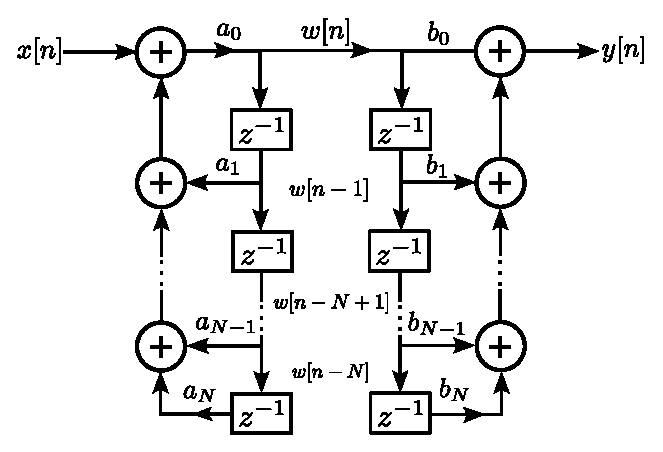
\includegraphics{images/IIR_filter.eps}
    \caption{Direct realisation of a digital IIR filter}
    \label{fig:IIR_direct}
\end{figure}

% Consider the following impulse response:
% \[
%     h[n] = b_0 a^{n} u[n] + b_1 a^{n-1} u[n-1]
% \]
% This is an infinite-length sequence, the filter is an infinite response filter. The system function thus
% \[
%     H(z) = \frac{b_0 + b_1 z^{-1}}{1 - az^{-1}}, \quad \lvert z \rvert > \lvert a \rvert
% \]
% Therefore, the system can also be seen as derived by the following difference equation:
% \[
%     y[n] - ay[n-1] = b_0 x[n] + b_1x[n-1]
% \]

% Structure for IIR filters
% \[
%     y[n] = \sum_{k=1}^{N} a_{k}y[n-k] + \sum_{k=0}^{M} b_{k}x[n-k]
% \]
% The general form for the system function is
% \[
%     H(z) = \frac{\sum_{k=0}^{M} b_{k} z^{-k}}{1 - \sum_{k=1}^{N} a_{k}z^{-k}}
% \]
% The output of the system in the $z$-domain is obtained as
% \[
%     Y(z) = H(z)X(z)
% \]
% or
% \[
%     Y(z) = \sum_{k=0}^{M} b_{k} b_{k} z^{-k} W(z), \quad \text{with} \quad W(z) = \frac{1}{1-\sum_{k=1}^{N} a_{k}z^{-k}}X(z)
% \]
The system function $H(z)$ can also be represented as a cascade of filters by factorizing the numerator and denominator:
\[
    H(z) = A \frac{\Pi_{k=1}^{M_1}(1-f_{k}z^{-1}) \Pi_{k=1}^{M_2}(1-g_{k}z^{-1})(1-g_{k}^{*}z^{-1})}{\Pi_{k=1}^{N_1}(1-c_{k}z^{-1}) \Pi_{k=1}^{N_2}(1-d_{k}z^{-1})(1-d_{k}^{*}z^{-1})}
\]


\subsubsection{IIR Filter Design by Bilinear Transformation}
The bilinear transformation transforms from the continuous-time systems in the Laplace domain to discrete-time systems in the $z$-domain. \\

An \textit{analogue} filter can always be described by a frequency domain system function of the general form, 
\[
    H(s) = \alpha\frac{(s-z_{1})(s-z_{2})...(s-z_{m})}{(s-p_{1})(s-p_{2})...(s-p_{n})}
\]
In bilinear transformation, we replace $s$ by $z$:
\[
    z = \frac{\alpha+s}{\alpha-s} \Leftrightarrow s 
    = \alpha \frac{z-1}{z+1} \bigg \lvert_{z=e^{j\omega}} 
    = \alpha \frac{e^{j\frac{\omega}{2}} - e^{-j\frac{\omega}{2}}}{e^{j\frac{\omega}{2}} + e^{-j\frac{\omega}{2}}} 
    = j\alpha\tan\frac{\omega}{2} = j\Omega
\]
Frequency mapping:
\[
    \Omega = \alpha \tan\frac{\omega}{2}
\]
Overall, the bilinear transformation allows the design of IIR filters from analogue filters: $H(s) \to H(\omega)$.

\newpage
\section{Random Processes}
%% subsection
\subsection{Statistical Descriptions of Noise and Random Processes}
Noise signals cannot be described analytically. However, noise realizations in a specific condition share some \textit{statistical} properties. \\

\textbf{Random process} is the collection of \textbf{random variables}, denoted by $\mathbf{x}_n$. The theory of probability can characterise random variables.

\paragraph{Probability Distribution Function} A random variable is characterized by its probability distribution function, $F_{\mathbf{x}_n}(\alpha, n)$,
\[
    F_{\mathbf{x}_n}(\alpha, n) = P\{\mathbf{x}_n\leq \alpha\}.
\]
Note that the probability density function increases monotonically with $\alpha$.

\paragraph{Probability Density Function} If $\mathbf{x}_{n}$ takes a continuous range of values, it can also be characterized by the probability density function, $f_{\mathbf{x}_n}(\alpha, n)$,
\[
    f_{\mathbf{x}_n}(\alpha, n) = \frac{\partial F_{\mathbf{x}_n}(\alpha, n)}{\partial \alpha}.
\]
%% subsubsection
\subsubsection{Mean and Variance of a Distribution}
\begin{enumerate}
    \item The probability density between the range $a$ and $b$ is found
        \begin{align*}
            P \{a \leq \mathbf{x}_n \leq b \} 
            & = \int_{a}^{b} f_{\mathbf{x}_n} (\alpha, n) \ \mathrm{d} \alpha \\
            & = F_{\mathbf{x}_n}(b, n) - F_{\mathbf{x}_n}(a, n).
        \end{align*}
        For $a = -\infty$ and $b = +\infty$,
        \[
            P \{-\infty \leq \mathbf{x}_n \leq +\infty \} = \int_{-\infty}^{+\infty} f_{\mathbf{x}_n} (x, n) \ \mathrm{d} x = 1
        \]

        \begin{ex}{Uniform distribution}
        \label{ex:uniform_dist}
            Consider the probability density function of a uniform distribution described as
            \[
                f_{\mathbf{x}_n} (\alpha, n) = 
                \begin{cases}
                    \frac{1}{b-a}, & a \leq \alpha \leq b \\
                    0, & \text{otherwise}
                \end{cases}, 
            \]
            the corresponding probability distribution is
            \[
                F_{\mathbf{x}_n} (\alpha, n) = 
                \begin{cases}
                    0, & a < 0 \\
                    \frac{1}{b-a}(\alpha-a), & a \leq \alpha \leq b \\
                    1, & \alpha > b
                \end{cases}.
            \]
            As shown in \autoref{fig:uniform_dist}.
            \begin{figure}[H]
                \centering
                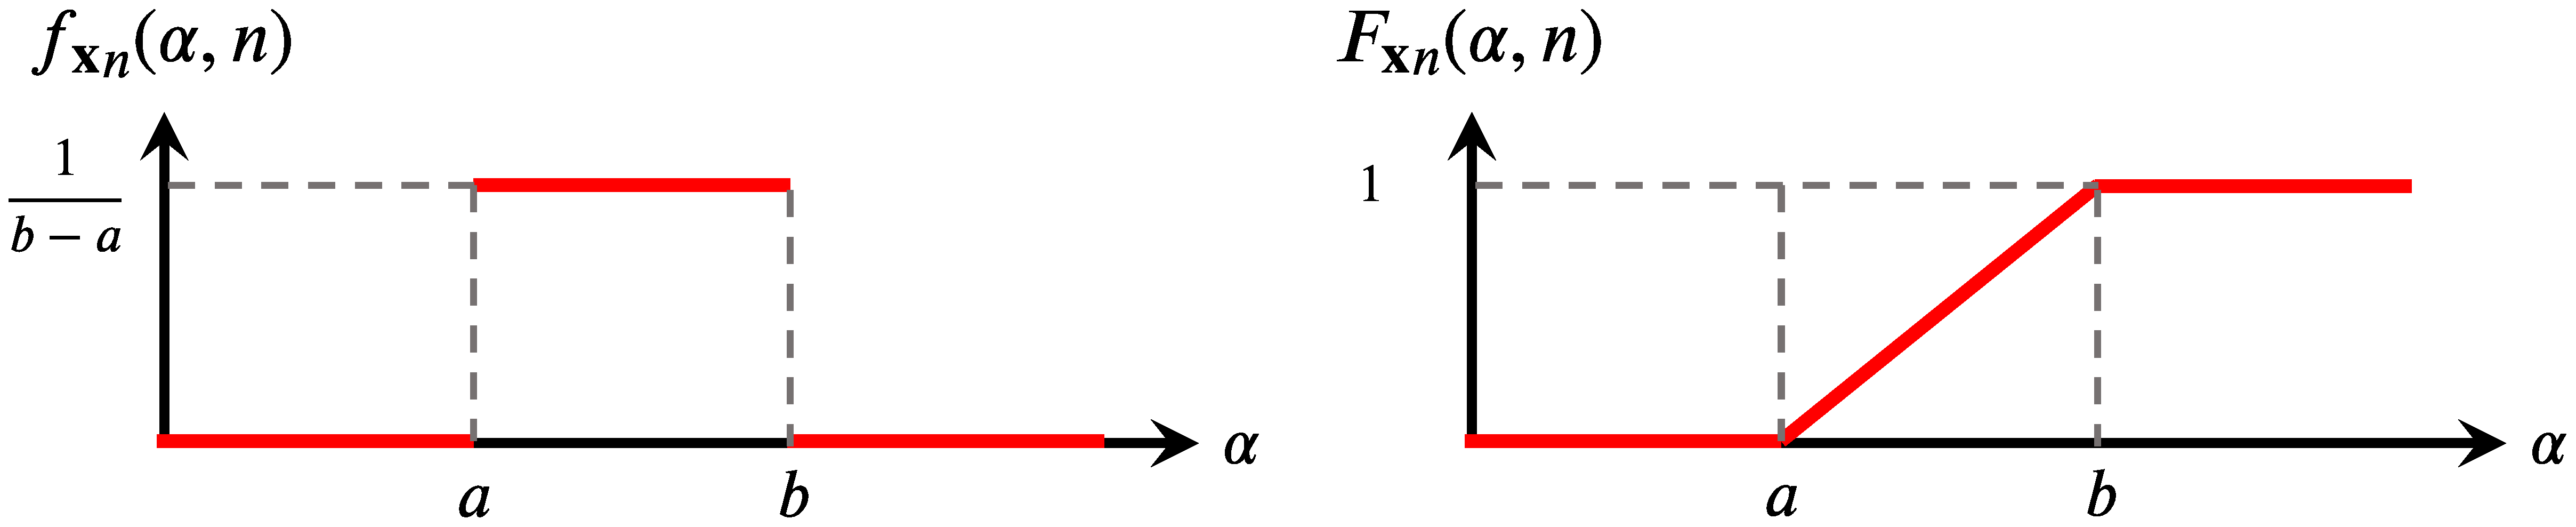
\includegraphics[width=\textwidth]{images/uniform_dist.eps}
                \caption{Plot of the probability density function and probability distribution function of a sample uniform distribution.}
                \label{fig:uniform_dist}
            \end{figure}
        \end{ex}

    \item The \textbf{mean} of a random variable, also the \textbf{expected value}, is defined as
    \[
        m_{\mathbf{x}_n} = \varepsilon\{\mathbf{x}_n\} = \int_{-\infty}^{+\infty} \alpha f_{\mathbf{x}_n}(\alpha, n) \ \mathrm{d}\alpha,
    \]
    where $\varepsilon\{\cdot\}$ denotes the \textbf{expectation operator}. Mathematically,
    \[
        \varepsilon \{ g(\mathbf{x}_n) \} = \int_{-\infty}^{+\infty} g(\alpha) f_{\mathbf{x}_n}(\alpha, n) \ \mathrm{d}\alpha.
    \]

    \begin{ex}{Uniform distribution}
        For the uniform distribution shown in \autoref{ex:uniform_dist}, the mean value is found
        \[
            m_{\mathbf{x}_n} = \int_{a}^{b} \frac{\alpha}{b-a} \ \mathrm{d}\alpha
            = \frac{1}{b-a}\frac{b^2 - a^2}{2} = \frac{a+b}{2}.
        \]
    \end{ex}

    \item The \textbf{variance} is define as
    \[
        \sigma_{\mathbf{x}_n}^2 
        = \varepsilon \{ (\mathbf{x}_n - m_{\mathbf{x}_n})^2 \} 
        = \int_{-\infty}^{+\infty} (\alpha - m_{\mathbf{x}_n})^2 f_{\mathbf{x}_n}(\alpha, n) \ \mathrm{d}\alpha,
    \]
    which is the second-order moment.
    
    \begin{ex}{Uniform distribution}
        For the uniform distribution shown in \autoref{ex:uniform_dist}, the variance is found
        \[
            \sigma_{\mathbf{x}_n}^2
            = \int_{a}^{b} \bigg(\alpha - \underbrace{\frac{a+b}{2}}_{m_{\mathbf{x}_n}}\bigg)^2 \frac{1}{b-a} \ \mathrm{d}\alpha
            = \frac{(b-a)^2}{12}.
        \]
    \end{ex}
\end{enumerate}

%% subsubsection
\subsubsection{Multivariant Probability Functions}
\paragraph{Joint Probability Distribution Function} The \textit{joint} probability distribution function between two random variables $\mathbf{x}_n$,  $\mathbf{x}_m$ is given as 
\[
    F_{\mathbf{x}_n, \mathbf{x}_m}(\alpha_1, \alpha_2, n,m) = P\{\mathbf{x}_n\leq \alpha_1, \mathbf{x}_m \leq \alpha_2\},
\]
The probability distribution function of order $N$ is given as
\[
    F_{\mathbf{x}_{n_1}, ..., \mathbf{x}_{n_N}} (\alpha_1, ..., \alpha_N, n_1, ..., n_N) = P(\mathbf{x}_{n_1} \leq \alpha_{1}, ..., \mathbf{x}_{n_N} \leq \alpha_{N}).
\]

\paragraph{Joint Probability Density Function} The \textit{joint} probability density function between two random variables $\mathbf{x}_n$,  $\mathbf{x}_m$ are given as
\[
    f_{\mathbf{x}_n, \mathbf{x}_m}(\alpha_1, \alpha_2, n,m) = \frac{\partial^2  F_{\mathbf{x}_n, \mathbf{x}_m}(\alpha_1, \alpha_2, n,m)}{\partial \alpha_1 \partial \alpha_2}.
\]
\begin{figure}[H]
    \centering
    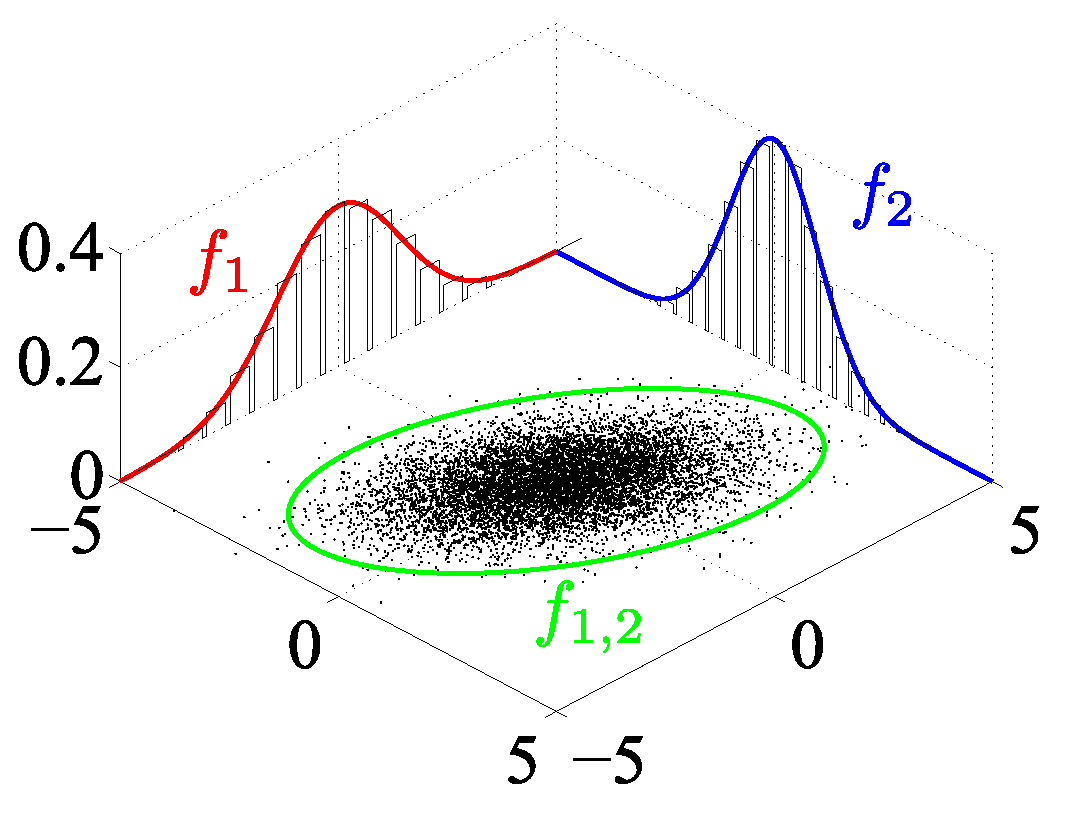
\includegraphics[scale=.5]{images/Multivariate_normal_sample.eps}
    \caption{Many sample observations (black) are shown from a joint probability distribution. Figure adapted and modified based on \href{https://en.wikipedia.org/wiki/Joint_probability_distribution\#/media/File:Multivariate_normal_sample.svg}{WikiPedia}.}
    \label{fig:joint_pdf}
\end{figure}

\paragraph{Statistical Independence} If $\mathbf{x}_n$ and $\mathbf{x}_m$ are \textbf{statistically independent}, or \textbf{uncorrelated}, the joint probability distribution function is equivalent to the product between each single probability distribution function,
\[
    F_{\mathbf{x}_n, \mathbf{x}_m}(\alpha_1, \alpha_2, n,m) = F_{\mathbf{x}_n}(\alpha_1, n)F_{\mathbf{x}_m}(\alpha_2, m),
\]
this also implies that
\[
    f_{\mathbf{x}_n, \mathbf{x}_m}(\alpha_1, \alpha_2, n,m) = f_{\mathbf{x}_n}(\alpha_1, n)f_{\mathbf{x}_m}(\alpha_2, m).
\]
Hence, the mean values are also separable,
\[
    \varepsilon\{\mathbf{x}_n \mathbf{x}_m\} = \varepsilon\{\mathbf{x}_n\}\varepsilon\{\mathbf{x}_m\} = m_{\mathbf{x}_n}m_{\mathbf{x}_m}.
\]

\paragraph{Autocorrelation Function} The autocorrelation function of the random process is defined as the expected value of the product $\mathbf{x}_n \mathbf{x}_m$, denoted by $\phi_{xx}[n,m]$,
\[
    \phi_{xx}[n,m] = \varepsilon\{ \mathbf{x}_n \mathbf{x}_m \}.
\]
\begin{ex}{\textbf{Uniform Distribution}}
    Given a random process with uncorrelated samples of uniform distribution in $[−1,1]$ (\textit{i.e.}, $a=-1$, $b=1$), the autocorrelation function computed with the following steps
    \begin{enumerate}
        \item The mean is found as
        \[
            m_{\mathbf{x}_n} = \frac{a+b}{2} = 0.
        \]

        \item The variance is found as
        \[
            \sigma_{\mathbf{x}_n}^2 = \frac{(b-a)^2}{12} = \frac{1}{3}.
        \]

        \item The autocorrelation between $m$ and $n$ is
        \[
            \phi_{xx}[n,m] 
            = \varepsilon\{ \mathbf{x}_n \mathbf{x}_m \} 
            = 
            \begin{cases}
                \varepsilon\{\mathbf{x}_n\}\varepsilon\{\mathbf{x}_m\}, & \text{if } m \neq n \\
                \varepsilon\{\mathbf{x}_n^2\}, & \text{if } m = n \\
            \end{cases}
            \ = \
            \begin{cases}
                0, & \text{if } m \neq n \\
               \frac{1}{3}, & \text{if } m = n \\
            \end{cases}.
        \]
    \end{enumerate}
\end{ex}

%% subsection
\subsection{Stationarity}
\paragraph{Definition}  A random process is \textbf{stationary} of order $N$, if its joint probability density functions up to order $N$, does not depend on time shifts.\\

For example, $N=2$, the stationarity states that 
\[
    F_{\mathbf{x}_{n+k}}(\alpha, n+k) = F_{\mathbf{x}_{n}}(\alpha, n), \quad \forall k \in \mathbb{Z},
\]
\[
    F_{\mathbf{x}_{n+k}, \mathbf{x}_{m+k}}(\alpha_1, \alpha_2, n+k, m+k) = F_{\mathbf{x}_{n}, \mathbf{x}_{m}}(\alpha_1, \alpha_2, n, m), \quad \forall k \in \mathbb{Z}.
\]

A random process is \textbf{strict-sense stationary} if it is stationary for \textit{any} order $N$.

\subsubsection{Wide-Sense Stationarity}
If the process is stationary of order 2 ($N=2$). The following two properties can be derived,
\begin{enumerate}
    \item its mean does not depend on time, \textit{i.e.},
        \[
            m_{\mathbf{x}_n} = \varepsilon\{\mathbf{x}_n\} = m_{\mathbf{x}}.
        \]
    \item the autocorrelation function depends only on the time difference, 
        \[
            \phi_{xx}[n, m] = \varepsilon\{ \mathbf{x}_n \mathbf{x}_m \} = \int_{-\infty}^{+\infty} \int_{-\infty}^{+\infty} \alpha_1 \alpha_2 f_{\mathbf{x}_n, \mathbf{x}_m} (\alpha_1 \alpha_2, n, m) \ \mathrm{d}\alpha_1 \mathrm{d}\alpha_2,
        \]
        now define $\ell = m-n$ (for which $\ell$ can be regarded as a time shift), we have $m = n + \ell$ 
        \begin{align*}
            \phi_{xx}[n, n+\ell]
            & = \varepsilon\{ \mathbf{x}_n \mathbf{x}_{n+\ell} \} = \int_{-\infty}^{+\infty} \int_{-\infty}^{+\infty} \alpha_1 \alpha_2 f_{\mathbf{x}_n, \mathbf{x}_{n+\ell}} (\alpha_1 \alpha_2, n, {n+\ell}) \ \mathrm{d}\alpha_1 \mathrm{d}\alpha_2\\
            & = \phi_{xx}[\ell].
        \end{align*}
\end{enumerate}
A process with the properties above is referred to as \textbf{wide-sense stationary} (WSS).\\

While the two above properties derive from the definition of stationarity of order 2, \textbf{they do not imply stationarity of order 2}.

\begin{ex}{Uniform Distribution}
A random signal with uncorrelated samples of uniform distribution in $[−a, a]$. The mean of the signal is
\[
    m_{\mathbf{x}_n} = \frac{-a + a}{2} = 0,
\]
and the autocorrelation function is
\[
    \phi_{xx}[n,m] = \frac{a^2}{3} \delta[n-m].
\]
Since the mean does not depend on $n$ and the autocorrelation function depends only on the time lag ($n-m$), the process is WSS.
\end{ex}

\paragraph{Cross-Correlation Function} The cross-correlation function is defined as 
\[
    \phi_{xy} [n,m] = \varepsilon\{\mathbf{x}_n \mathbf{y}_m^*\},
\]
where $\mathbf{x}_n$ and $\mathbf{y}_n$ are two distinct random signals.

%% subsection
\begin{mdframed}[frametitle={Chnage in notation}, nobreak=false]
    From this subsection onward, the random variable at the discrete-time $n$ will be denoted as $x[n]$, instead of $\mathbf{x}_n$.
\end{mdframed}
\subsection{Ergodicity}
\paragraph{Definition}  A process is \textbf{ergodic} for the mean (time-average) if, for any single realization of the process of $x[n]$,
\[
    \langle x[n] \rangle = \lim_{L\to \infty} \frac{1}{2L+1} \sum_{n=-L}^{L} x[n] = \varepsilon\{\mathbf{x}_n\} = m_{x}.
\]

\paragraph{Extended Properties} A process is ergodic for the autocorrelation of
\[
    \langle x[n] x[n+m] \rangle = \lim_{L\to\infty} \frac{1}{2L+1} \sum_{n=-L}^{L} x[n] x[n+m] = \varepsilon\{\mathbf{x}_{n}\mathbf{x}_{n+m}\} = \phi_{xx}[m].
\]

For a WSS random process, ergodic for the autocorrelation function is
\[
    \langle x^2[n] \rangle = \lim_{L\to\infty} \frac{1}{2L+1} \sum_{n=-L}^{L} x^2[n] = \phi_{xx}[0].
\]
The value of the autocorrelation function is zero for an ergodic process corresponds to the power of each of the process realizations.\\

If the process is zero-mean, 
\[
    \lim_{L\to\infty} \frac{1}{2L+1}\sum_{n=-L}^{L} x^2[n] = \phi_{xx}[0] = \sigma_{\mathbf{x}_n}^2.
\]

%% subsubsection
\subsubsection{Variability of Estimates}
In practice, we cannot compute the exact time average since we do not record infinite samples. Thus, we need to make estimates\footnote{such estimated quantities are denoted with a superscript caret, $\widehat{\text{ }}$, to distinguish from the real values} from a finite-length realisation.
\begin{itemize}
    \item Estimating the mean:
    \[
        \widehat{m}_{x} = \frac{1}{L} \sum_{n=0}^{L-1} x[n].
    \]

    \item Estimating the variance:
    \[
        \widehat{\sigma}_x^2 = \frac{1}{L} \sum_{n=0}^{L-1} (x[n] - \widehat{m}_{x})^2.
    \]

    \item Estimating the autocorrelation function:
    \[
        \widehat{\phi}_{xx}[m] = \frac{1}{L}\sum_{n=0}^{L-m-1} \ x[n] \ x[n+m].
    \]
\end{itemize}
The quantities, $\widehat{m}_{x}$, $\widehat{\sigma}_x^2$, and $\widehat{\phi}_{xx}[m]$ are also \textit{random} variables. Hence, we can compute the mean and variability of these estimated quantities. 

\begin{itemize}
    \item The mean of the estimated mean with a finite length:
    \[
        \varepsilon\{\widehat{m}_{x}\} = \varepsilon\bigg\{\frac{1}{L} \sum_{n=0}^{L-1} x[n] \bigg\} = \frac{1}{L} \sum_{n=0}^{L-1} \varepsilon\{x[n]\} = m_x,
    \]
    this means the estimated mean is \textbf{unbiased}.

    \item The variability of the estimated mean with a finite length (for simplicity, assume the true mean $m_x = 0$):
    \[
        \sigma_{\widehat{m}_{x}}^2 = \varepsilon\{(\widehat{m}_{x} - \varepsilon\{\widehat{m}_{x}\})^2\} =  \varepsilon\{(\widehat{m}_{x} - m_x)^2\} = \varepsilon \bigg\{\bigg(\frac{1}{L} \sum_{n=0}^{L-1} x[n]\bigg)^2\bigg\} = \frac{\sigma_x^2}{L}.
    \]
\end{itemize}

\paragraph{Variability in Estimates of the Autocorrelation Function} The estimate of the autocorrelation function in the finite-length realization is a \textbf{biased} estimate.
\[
    \varepsilon\{\widehat{\phi}_{xx}[m]\} = \frac{1}{L}\sum_{n=0}^{L-m-1} \ \varepsilon\{x[n] \ x[n+m] \} = \frac{L-m}{L} \phi_{xx}[m] = \underbrace{(1-\frac{m}{L})}_{\text{deviation from truth}}\phi_{xx}[m].
\]
To fix this, an alternative estimator is proposed to eliminate the bias,
\[
    \widehat{\phi}_{xx}[m] = \frac{1}{L-m}\sum_{n=0}^{L-m-1} \ x[n] \ x[n+m].
\]

%% subsection
\subsection{Power Spectral Density}
\paragraph{Definition} The power spectral density (PSD) of a random process is the ensemble average of the power spectrum of the random process realizations,
\[
    \Phi_{xx} (e^{j\omega}) = \varepsilon \bigg\{ \lim_{L\to\infty} \frac{1}{2L+1} \lvert X_{L}(e^{j\omega}) \rvert^2 \bigg\},
\]
where $X_{L}(e^{j\omega}) = \sum_{n=-L}^{L} x[n] e^{-j\omega n}$ is the Fourier transform of the random variable $x[n]$.

\paragraph{Signal Power} The power spectral density of an ergodic random signal,
\[ 
    \text{signal power} = \frac{1}{2\pi} \int_{-\pi}^{+\pi} \Phi_{xx}(e^{j\omega}) \mathrm{d}\omega
\]
\begin{dv}{}
Start from the RHS of the equation shown above,
\begin{align*}
    & \frac{1}{2\pi} \int_{-\pi}^{+\pi} \Phi_{xx}(e^{j\omega}) \mathrm{d}\omega \\
    & = \frac{1}{2\pi} \int_{-\pi}^{+\pi} \varepsilon \bigg\{ \lim_{L\to \infty} \frac{1} {2L+1} \lvert X_L (e^{j\omega}) \rvert^2 \bigg \} \mathrm{d}\omega \\
    & = \varepsilon \bigg\{ \lim_{L\to \infty} \frac{1} {2L+1} \ \frac{1}{2\pi} \int_{-\pi}^{+\pi} \lvert X_L (e^{j\omega}) \rvert^2 \mathrm{d}\omega \bigg\}.
\end{align*}
By Parseval's theorem:
\[
    \frac{1}{2\pi} \int_{-\infty}^{+\infty} \lvert X(e^{j\omega}) \rvert^2 \mathrm{d}\omega = \sum_{n=-\infty}^{+\infty} \lvert x[n] \rvert^2.
\]
Therefore, 
\[
    \frac{1}{2\pi} \int_{-\pi}^{+\pi} \Phi_{xx}(e^{j\omega}) \mathrm{d}\omega = \varepsilon \bigg\{ \lim_{L\to \infty} \frac{1} {2L+1} \ \sum_{n=-\infty}^{+\infty} \lvert x[n] \rvert^2 \bigg\},
\]
which is the power of the signal.
\end{dv}

\paragraph{Extended Property} The power spectral density of a WSS random process is the discrete-time Fourier transform (DTFT) of the autocorrelation function,
\[
    \Phi_{xx}(e^{j\omega}) = \mathcal{F} \{\phi_{xx}[m]\},
\]
where $\mathcal{F}\{\cdot\}$ denotes the discrete-time Fourier transform.
\begin{dv}{}
\begin{align*}
    \lvert X_{L}(e^{j\omega})\rvert^2 
    & = X_L(e^{j\omega}) X_L^{*}(e^{j\omega}) \\
    & = \sum_{n=-L}^{L} \sum_{r=-L}^{L} x[n] x^{*}[r] e^{-j\omega (n-r)}.
\end{align*}    
Therefore,
\begin{align*}
    \Phi_{xx}(e^{j\omega}) 
    & = \lim_{L\to\infty} \varepsilon \bigg\{ \frac{1}{2L+1} \sum_{n=-L}^{L} \sum_{r=-L}^{L} x[n] x^{*}[r] e^{-j\omega (n-r)} \bigg\} \\
    & = \lim_{L\to \infty} \bigg\{ \frac{1}{2L+1} \sum_{n=-L}^{L} \sum_{r=-L}^{L} \varepsilon \{ x[n] x^{*}[r] e^{-j\omega (n-r)} \} \bigg \}.
\end{align*}
For a WSS random signal,
\[
    \varepsilon \{ x[n] x^{*}[r] \} = \phi_{xx}[n, r] = \phi_{xx}[n-r].
\]
Therefore,
\[
    \Phi_{xx}(e^{j\omega}) = \lim_{L\to \infty} \bigg\{ \frac{1}{2L+1} \sum_{n=-L}^{L} \sum_{r=-L}^{L} \varepsilon \{ \phi_{xx}[n-r] e^{-j\omega (n-r)} \} \bigg \} = \mathcal{F}\{\phi_{xx}[m]\}.
\]
\end{dv}

Therefore, for a WSS and ergodic random signal,
\[
    \Phi(e^{j\omega}) = \mathcal{F} \bigg\{ \lim_{L\to\infty} \frac{1}{2L+1} \sum_{n=-L}^{L} x[n] \ x[n+m] \bigg\}.
\]
This tells us, the PSD is the discrete-time Fourier transform of the autocorrelation function of the process.

%% subsection
\subsection{Periodogram}
\paragraph{Definition} The periodogram is an estimation of the PSD with the limit neglected. 
\[
    \widehat{\Phi}_{xx} (e^{j\omega}) = \frac{1}{2L+1} \lvert X_{L} (e^{j\omega}) \rvert^2
\]
Therefore, it can be shown that the estimation of PSD from the periodogram and from the autocorrelation function is exactly the same:
\[
    \widehat{\Phi}_{xx}(e^{j\omega}) = DTFT \bigg\{ \frac{1}{2L+1} \sum_{n=-L}^{n=L} x[n] \ x[n+m] \bigg\} = DTFT \{ \widehat{\phi}_{xx}[m] \} = \frac{1}{2L+1} \lvert X_{L}(e^{j\omega})\rvert^2
\]
\paragraph{Bias of the Periodogram Estimate}
The expected value of the bias is
\[
    \varepsilon\{\widehat{\Phi}_{xx}(e^{j\omega})\} = \varepsilon \bigg\{ \frac{1}{2L+1} \lvert X_{L}(e^{j\omega})\rvert^2 \bigg\}
\]
This is equivalent to
\[
    x_{L}[n] = 
    \begin{cases}
        x[n], & -L \leq n \leq L \\
        0, & \text{otherwise} \\
    \end{cases}
    = x[n] \cdot w_{2L+1}[n]
    \quad \text{with} \quad 
    w_{2L+1}[n] = 
    \begin{cases}
        1, & -L\leq n\leq L \\
        0, & \text{otherwise} \\
    \end{cases}
\]
Therefore, the periodogram is a biased estimate. The estimate tends to the PSD of the windowed random signal,
\[
    \varepsilon \{ \widehat{\Phi}_{xx}(e^{j\omega}) \} = \Phi_{xx}(e^{j\omega}) * \lvert W_{2L+1}(e^{j\omega}) \rvert^2
\]

\paragraph{Bartlett's Method}
A major problem of the periodogram is \textbf{the variance of the estimate of the PSD is proportional to the square of the PSD value} and \textbf{remains constant with increasing $L$}. \\

To mitigate this issue, we need a compromise between the bias and variance of the estimate. With $N$ recorded samples, one could compromise the bias by dividing $N$ by the number of intervals $K$, yielding $L = N/K$. \\

Thus, we can estimate a periodogram by summing multiple ``piecewise'' periodograms on each interval:

\[
    \widehat{\Phi}_{xx}^B (e^{j\omega}) = \frac{1}{K} \sum_{r=1}^{K} \hat{\Phi}_{x_{r}x_{r}} (e^{j\omega}) \quad \text{with} \quad \hat{\Phi}_{x_{r}x_{r}} = \frac{1}{L} \lvert X_{r} (e^{j\omega}) \rvert^2
\]

The expected values of the periodograms:
\[
    \varepsilon\{\widehat{\Phi}_{xx}^{B} (e^{j\omega})\}
    = \varepsilon\bigg\{ \frac{1}{K} \sum_{r=1}^{K} \widehat{\Phi}_{x_{r}x_{r}} (e^{j\omega}) \bigg\} = \Phi_{xx}(e^{j\omega}) * \lvert W_{2L+1}(e^{j\omega}) \rvert^2
\]
The variance of the periodograms:
\[
    var\{\widehat{\Phi}_{xx}^{B} (e^{j\omega})\} = var \bigg\{ \frac{1}{K} \sum_{r=1}^{K} \widehat{\Phi}_{x_{r}x_{r}} (e^{j\omega}) \bigg\} = \frac{1}{K} var\{\widehat{\Phi}_{xx}(e^{j\omega}) \}
\]
The variance of the estimation decreases as $K$ increases. 

\subsection{Filtering of Random Signals}
\[
    y[n] = x[n] * h[n] = \sum_{k=-\infty}^{+\infty} x[k] h[n-k] = \sum_{k=-\infty}^{+\infty} h[k]x[n-k]
\]
\paragraph{Mean of $y[n]$}
\[
    m_y[n] = \varepsilon\bigg\{ \sum_{k=-\infty}^{+\infty} x[k] h[n-k] \bigg\} = \sum_{k=-\infty}^{+\infty} h[k] \varepsilon\{x[n-k]\} = m_x \sum_{k=-\infty}^{+\infty} h[k]
\]
\paragraph{Autocorrelation function of $y[n]$}
\begin{align*}
    \phi_{yy}[n,\ell] 
    & = \varepsilon \{ y[n] \ y[n+\ell] \} \\
    & = \varepsilon \bigg\{ \sum_{k=-\infty}^{+\infty} h[k]x[n-k] \sum_{k=-\infty}^{+\infty} h[k] x[n+\ell-k] \bigg\} \\
    & = \varepsilon \bigg\{ \sum_{k=-\infty}^{+\infty} \sum_{r=-\infty}^{+\infty} h[k] \ h[r] \ x[n-k] \ x[n+\ell-r] \bigg\} \\
    & = \sum_{k=-\infty}^{+\infty} \sum_{r=-\infty}^{+\infty} h[k] \ h[r] \ \varepsilon \{ x[n-k] \ x[n+\ell-r] \} \\
    & = \sum_{k=-\infty}^{+\infty} \sum_{r=-\infty}^{+\infty} h[k] \ h[r] \ \phi_{xx}[\underbrace{\ell-r+k}_{\text{def.} \ r-k = q}] \\
    & = \sum_{k=-\infty}^{+\infty} \sum_{q=-\infty}^{+\infty} h[k] \ h[k+q] \ \phi_{xx}[\ell-q] \\
    & \hspace{-1cm} (\color{gray}\text{define} \ g[q] = \sum_{k=\infty}^{+\infty}h[k] \ h[k+q] = h[q] * h[-q]) \\
    & = \sum_{q=-\infty}^{+\infty} g[q] \phi_{xx}[\ell-q] = g[\ell]*\phi_{xx}[\ell] = \phi_{yy}[\ell]
\end{align*}

\paragraph{PSD of $y[n]$}
The PSD of $y[n]$ is the discrete-time FT of the autocorrelation function $\phi_{yy}[\ell]$,
\[
    \phi_{yy}[\ell] = g[\ell] * \phi_{xx}[\ell]
\]
with $g[q] = h[q] * h[-q]$,
\[  
    \Phi_{yy}(e^{j\omega}) = \mathcal{F} \{ g[\ell] * \phi_{xx}[\ell] \} = G(e^{j\omega}) \cdot \Phi_{xx} (e^{j\omega})
\]
with 
\[
    G(e^{j\omega}) = \mathcal{F} \{ h[q] *h[-q] \} = H(e^{j\omega}) \cdot H^{*}(e^{j\omega}) = \lvert H(e^{j\omega}) \rvert^2
\]
Therefore, 
\[
    \Phi_{yy}(e^{j\omega}) = \lvert H(e^{j\omega}) \rvert^2 \cdot \Phi_{xx}(e^{j\omega})
\]

\subsection{Linear Predictor}
The mean square error for the linear predictor
\[
    \varepsilon\{\lvert e[n] \rvert^2\} = \varepsilon \bigg\{ \bigg( x[n] - \sum_{k=1}^{N} a_k x[n-k] \bigg)^2 \bigg\} = \phi_{xx}[0] + \sum_{k=1}^{N}\sum_{r=1}^N a_k a_r \phi_{xx}[r-k] - 2 \sum_{k=1}^N a_k \phi_{xx}[k]
\]
Minimising the MSE,
\[
    \frac{\partial \varepsilon\{\lvert e[n] \rvert^2\}}{\partial a_{\ell}} = 0, \quad \ell = 1, 2,..., N
\]
with
\[
    \frac{\partial \varepsilon\{\lvert e[n] \rvert^2\}}{\partial a_{\ell}} = 2\sum_{k=1}^N a_k \phi_{xx}[k-\ell] - 2\phi_{xx}[\ell]
\]
Hence
\[
    2\sum_{k=1}^N a_k \phi_{xx}[k-\ell] - 2\phi_{xx}[\ell] = 0 
    \quad \Rightarrow \quad
    \boxed{\sum_{k=1}^N a_k \phi_{xx}[k-\ell] = \phi_{xx}[\ell]}
\]
which is equivalent to
\[
    \varepsilon \{e[n] \ x[n-k] \} = 0, \quad k = 1, 2, ..., N
\]
The error in the linear prediction can thus be seen as part of the innovation of the process that is not contained in the previous $N$ samples.

\subsection{Modelling}
Consider an LTI system with the input $u[n]$, system function $H(e^{j\omega})$, and output $x[n]$, for which $u[n]$ is a white random process.
\begin{figure}[H]
    \centering
    \begin{tikzpicture}[auto, node distance=2.2cm, >=Latex]
        % Nodes
        \node (input) {$u[n]$};
        \node [draw, line width=0.25mm, rectangle, minimum width=1.5cm, minimum height=0.7cm, right=.7cm of input] (block1) {$H(e^{^{j\omega}})$};
        \node [right=0.7cm of block1] (output) {$x[n]$};
        % Arrows
        \draw[line width=0.25mm, ->] (input) -- (block1);
        \draw[line width=0.25mm, ->] (block1) -- (output);
    \end{tikzpicture}
\end{figure}
Recall that in Section 5, the system response can be expressed using the difference equation
\[
    x[n] = \sum_{k=1}^{N} a_{k}x[n-k] + \sum_{k=0}^{M} b_{k}u[n-k].
\]
Further, the system function corresponding to the difference form is
\[
    H(z) = \frac{\sum_{k=0}^{M} b_{k} z^{-k}}{1-\sum_{k=1}^{N} a_{k} z^{-k}}
    \quad \Leftrightarrow \quad
    H(e^{j\omega}) = \frac{\sum_{k=0}^M b_k e^{-j\omega k}}{1-\sum_{k=1}^N a_k e^{-j\omega k}},
\]

Therefore, the power spectrum of $x[n]$ is found
\[
    \Phi_{xx}(e^{j\omega}) = \sigma_u^2 \cdot \lvert H(e^{j\omega}) \rvert^2 = \sigma_u^2 \cdot \bigg \lvert \frac{\sum_{k=0}^M b_k e^{-j\omega k}}{1-\sum_{k=1}^N a_k e^{-j\omega k}} \bigg\rvert^2 . 
\]
This model is known as the \textbf{autoregressive, moving average} model (ARMA).
\begin{itemize}
    \item By setting $M = 0$: autoregressive (AR) model
    \[
        x[n] = \sum_{k=1}^{N} a_{k}x[n-k] + u[n]
        \quad \text{and} \quad
        \Phi_{xx}(e^{j\omega}) = \sigma_u^2 \cdot  \frac{1}{\lvert 1-\sum_{k=1}^N a_k e^{-j\omega k}\rvert^2}
    \]

    \item By setting $N = 0$: moving average (MA) model
    \[
        x[n] = \sum_{k=0}^{M} b_{k}u[n-k]
        \quad \text{and} \quad
        \Phi_{xx}(e^{j\omega}) = \sigma_u^2 \cdot  \left\vert \sum_{k=0}^M b_k e^{-j\omega k} \right\vert^2
    \]
\end{itemize}

\subsection{Example Questions}
%==============================================%
\begin{q}{}
Let $x[n]$ and $y[n]$ be stationary, uncorrelated to each other, discrete-time random processes with mean values $m_x$ and $m_y$, respectively, and $w[n] = x[n] \cdot y[n]$. The mean value of $w[n]$ is

\begin{enumerate}[label=(\alph*)]
    \item Always zero
    \item Zero only of $m_x = 0$ and $m_y = 0$
    \item Zero if $m_x = 0$ or $m_y = 0$
    \item Always smaller than $m_x$
    \item Always smaller than $m_y$
\end{enumerate}
\begin{flushright}
    \begin{blueenv}
        ANS: (c)
    \end{blueenv}
\end{flushright}
\end{q}
%==============================================%
\begin{q}{}
Let $x[n]$ and $y[n]$ be two stationary, zero-mean, uncorrelated to each other, discrete-time random processes, with variances $\sigma_x^2$ and $\sigma_y^2$, and power spectra $\Phi_{xx}(e^{j\omega})$ and $\Phi_{yy}(e^{j\omega})$, respectively.\\

Let's define the random process $w[n] = x[n] + 2y[n]$, with variance $\sigma_w^2$ and power spectrum $\Phi_{ww}(e^{j\omega})$. Which of the following relations is always correct?

\begin{enumerate}[label=(\alph*)]
    \item $\Phi_{ww}(e^{j\omega}) = 2\Phi_{xx}(e^{j\omega}) \Phi_{yy}(e^{j\omega})$
    \item $\Phi_{ww}(e^{j\omega}) = \Phi_{xx}(e^{j\omega}) + 2\Phi_{yy}(e^{j\omega})$
    \item $\sigma_w^2 = \sigma_x^2 + 2\sigma_y^2$
    \item $\sigma_w^2 = \sigma_x^2 + 4\sigma_y^2$
    \item $\sigma_w^2 = 0$
\end{enumerate}
\begin{flushright}
    \begin{blueenv}
        ANS: (d)
    \end{blueenv}
\end{flushright}
\end{q}
%==============================================%
\begin{q}{}
Consider the wide-sense stationary (WSS) random process $x[n]$, with autocorrelation function $\phi_{xx}[\ell]$ and unitary variance. The autocorrelation function $\phi_{xx}[\ell]$ is equal to zero for all values of the time lag $\ell$ for which $|\ell| \geq 3$. The random process $x[n]$ is down-sampled by a factor of 3 to obtain the down-sampled random process $e[n]$. Which of the following expressions/statements for the autocorrelation function $\phi_{ee}[\ell]$ of $e[n]$ is correct?

\begin{enumerate}[label=(\alph*)]
    \item $\phi_{ee}[\ell] = \delta[\ell]$
    \item $\phi_{ee}[\ell] = \phi_{xx}[\ell]$
    \item $\phi_{ee}[\ell] = 3\phi_{xx}[\ell]$
    \item $\phi_{ee}[\ell] = 0$ for all values of $\ell$
    \item $\phi_{ee}[\ell]$ is an odd function
\end{enumerate}

\begin{flushright}
    \begin{blueenv}
        ANS: (d)
    \end{blueenv}
\end{flushright}
\end{q}
%==============================================%
\begin{q}{}
Consider the cascade of two LTI systems as represented below:
\begin{figure}[H]
    \centering
    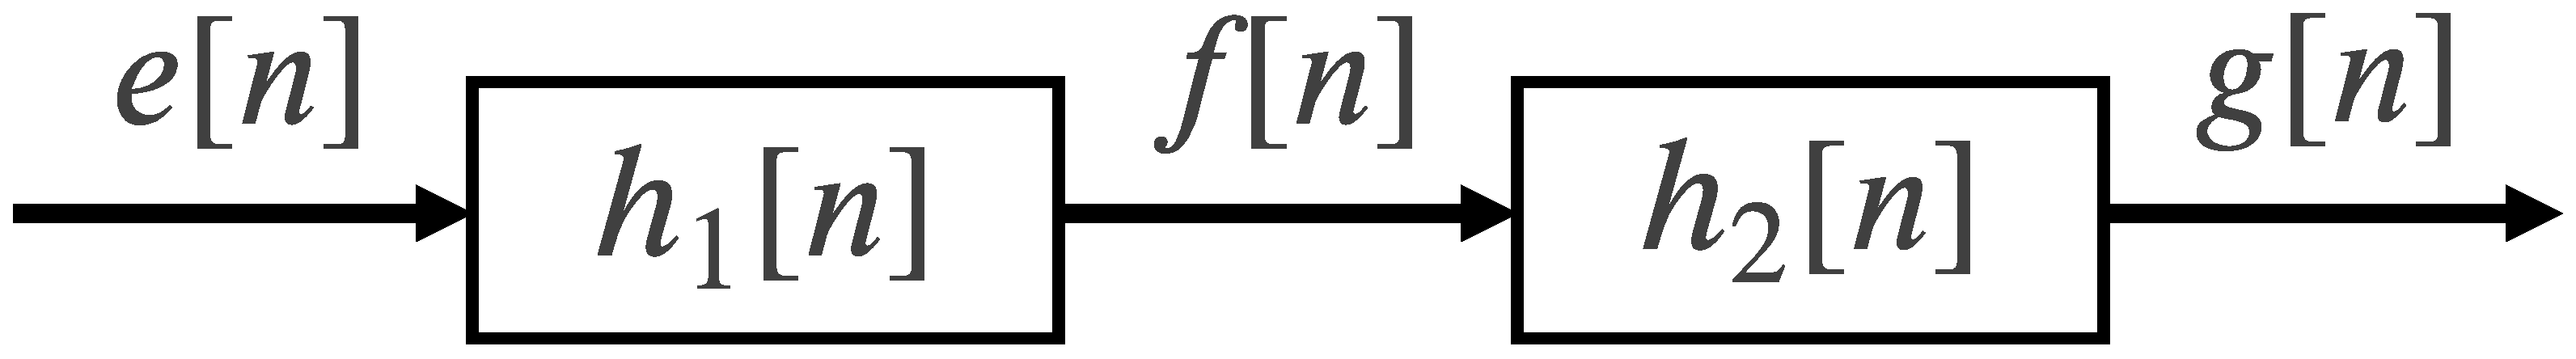
\includegraphics[width=.5\textwidth]{images/random_proc_ex.eps}
\end{figure}
where $h_1[n] = \delta[n] - \delta[n-1]$ and $\displaystyle H_2(e^{j\omega}) = \begin{cases}
1, \quad \lvert \omega \rvert < \omega_c \\
0, \quad \omega_c < \lvert \omega \rvert \leq \pi
\end{cases}
$ with $\omega_{c} < \pi$. Moreover, $e[n]$ is a stationary, white random signal, with zero mean and power $\sigma_{e}^2 = 1$.

\begin{enumerate}[label=(\alph*)]
    \item Find and plot the power spectrum $\Phi_{ff}(e^{j\omega})$ of the random signal $f[n]$.

    \begin{flushright}
        \begin{blueenv}
            ANS: $\Phi_{ff}(e^{j\omega}) = 2 (1 - \cos\omega)$.
        \end{blueenv}
    \end{flushright}

    \item Find the autocorrelation function $\phi_{ff}[\ell]$ of the random signal.
    \begin{flushright}
        \begin{blueenv}
            ANS: $\phi_{ff}[\ell] = 2\delta[\ell] - \delta[\ell-1] - \delta[\ell + 1]$.
        \end{blueenv}
    \end{flushright}

    \item Find the power spectrum $\Phi_{gg}(e^{j\omega})$ of the random signal $g[n]$ as a function of $\omega_c$ (cut-off frequency of the second LTI system).
    \begin{flushright}
        \begin{blueenv}
            ANS: $\phi_{gg}[\ell] = 
            \begin{cases}
            2(1-\cos\omega), & \lvert \omega \rvert \leq \omega_c \\
            0, & \omega_c < \lvert \omega \rvert \leq \pi
            \end{cases}$.
        \end{blueenv}
    \end{flushright}

    \item Find the power $\sigma_{e}^{2}$ of the random signal $g[n]$ as a function of $\omega_c$ (cut-off frequency of the second LTI system).
    \begin{flushright}
        \begin{blueenv}
            ANS: $\sigma_{g}^2 = \dfrac{2\omega_c}{\pi}$.
        \end{blueenv}
    \end{flushright}
\end{enumerate}

% \begin{blueenv}
% \paragraph{Answer (a)}
% \[
%     \Phi_{ff}(e^{j\omega}) = \Phi_{ee}(e^{j\omega}) \cdot \lvert H_1(e^{j\omega})\rvert^2,
% \]
% with
% \begin{itemize}
%     \item $\Phi_{ee}(e^{j\omega}) = 1$, 
%     \item $h_1[n] \ \xrightarrow[]{\mathcal{F}}H_1(e^{j\omega}) = 1 - e^{-j\omega} \quad \Rightarrow \quad \lvert H_1(e^{j\omega})\rvert^2 = 2 (1 - \cos\omega)$.
% \end{itemize}
% Hence, $\Phi_{ff}(e^{j\omega}) = 2 (1 - \cos\omega)$.

% \paragraph{Answer (b)} Given
% \[
%     f[n] = e[n] - e[n-1],
% \]
% hence,
% \begin{align*}
%     \phi_{ff}[\ell] 
%     & = \varepsilon \{f[n] \ f[n+\ell]\} \\
%     & = \varepsilon \{(e[n] - e[n-1])(e[n+\ell] - e[n+\ell-1])\} \\
%     & = 2 \phi_{ee}[\ell] - \phi_{ee}[\ell-1] - \phi_{ee}[\ell+1] \\
%     & = 2\delta[\ell] - \delta[\ell-1] - \delta[\ell + 1]
% \end{align*}

% \paragraph{Answer (c)}
% \[
%     \Phi_{gg}(e^{j\omega}) = \Phi_{ff}(e^{j\omega}) \lvert H_2(e^{j\omega}) \rvert^2 = 
%     \begin{cases}
%         2(1-\cos\omega), & \lvert \omega \rvert \leq \omega_c \\
%         0, & \omega_c < \lvert \omega \rvert \leq \pi
%     \end{cases}
% \]

% \paragraph{Answer (d)}
% \begin{align*}
%     \sigma_{g}^2
%     & = \frac{1}{2\pi} \int_{-\infty}^{+\infty} \Phi_{gg}(e^{j\omega}) \mathrm{d}\omega \\
%     & = \frac{1}{2\pi} \int_{-\omega_c}^{+\omega_c} 2(1-\cos\omega) \mathrm{d}\omega \\
%     & = \frac{1}{2\pi} (4\omega_c - 2\sin\omega_c + 2\sin\omega_c) \\
%     & = \frac{2\omega_c}{\pi}
% \end{align*}
% \end{blueenv}
    
\end{q}

\newpage
\thispagestyle{empty}
\newgeometry{margin=1.8cm}
\mbox{}
\vfill    
\begin{figure}[H]
    \includegraphics[right]{images/by-nc.eps}
\end{figure}
\textit{This work is licensed under a Creative Commons Attribution-NonCommercial 4.0 International License.}


\end{document}
